\chapter{Architectural Design} \label{chap2}
The System Architecture is a way to give the overall view of a system and to put it in relation to external systems. This allows the reader to have a more complete and general idea of the entire system and at the same time to have a deeper view of the principal components of the system itself.

\section{Overview}
This section provides a general description of the architecture of the system.
The system has a 4-tier architecture, following the common Java EE architecture, in which the presentation relies upon the client machines, the server machine takes care of the business logic and the web tier and the database is on a dedicated machine.
In this document the web application and the Android mobile application are treated as one entity, so all the communication between client and server will pass through the Web Tier. JSF technology will be used for dynamic web pages and an implementation of the REST paradigm will be assumed for communicating with the Android app.

More in details JEE has a four tiered architecture divided as:
\begin{itemize}
	\item \textbf{Client Tier}: This tier contains Application Clients and Web Browsers, and it is the layer that interacts directly with the actors.
	\item \textbf{Web Tier}: This tier will manage all the requests that are send by the client, generating the corresponding messages that the business tier will need to process the information. This tier also will send back the answer of the request to the Client Tier, so it can be shown to the user. 
	\item \textbf{Business Tier}: This tier is composed by the Enterprise Java Beans, which manage all the system logic and Java Persistence Entities. The Java Beans will also manage the different types of users that can access to a certain page or information. All the information data will be retrieved from the database.
	\item \textbf{Data Tier}: This tier contains the data source. It is the database allowed to store all the relevant data and to retrieve them.
\end{itemize}

\begin{figure}[htbp]
\centering
\includegraphics[width=\textwidth]{cpt/img/JavaEEOverview}
\caption{JEE 4-tier architecture}
\end{figure}
\clearpage

\section{High Level Components and their Interaction}
The diagram in Figure \ref{fig:HLC}  represents our conceptual design of MyTaxiService. This diagram depicts all the components of the designed software.
The Client Tier is composed of the interfaces of the different users in order to allow to each user to see the correct XHTML or Mobile App pages. Actually this is strictly related to the Web Tier, which is composed of the web beans. This Tier receives the requests of the user and has some specific beans which listen to these events and display data regarding the user requests. They interact with the beans in Business Tier, to retrieve the information. Since the system is using JSF these beans are called Managed Beans.
The Business Logic Tier is composed of all the logic underlying the application; it is
responsible of communication with Web Tier and the Java Persistence and its components are the EJB Beans.
The Java Persistence is composed of the entity beans that are fundamental as they represent the connection to the Database. In Java Enterprise Environment they represent a high level object view of the Database of the application.

\begin{figure}[htbp]
\centering
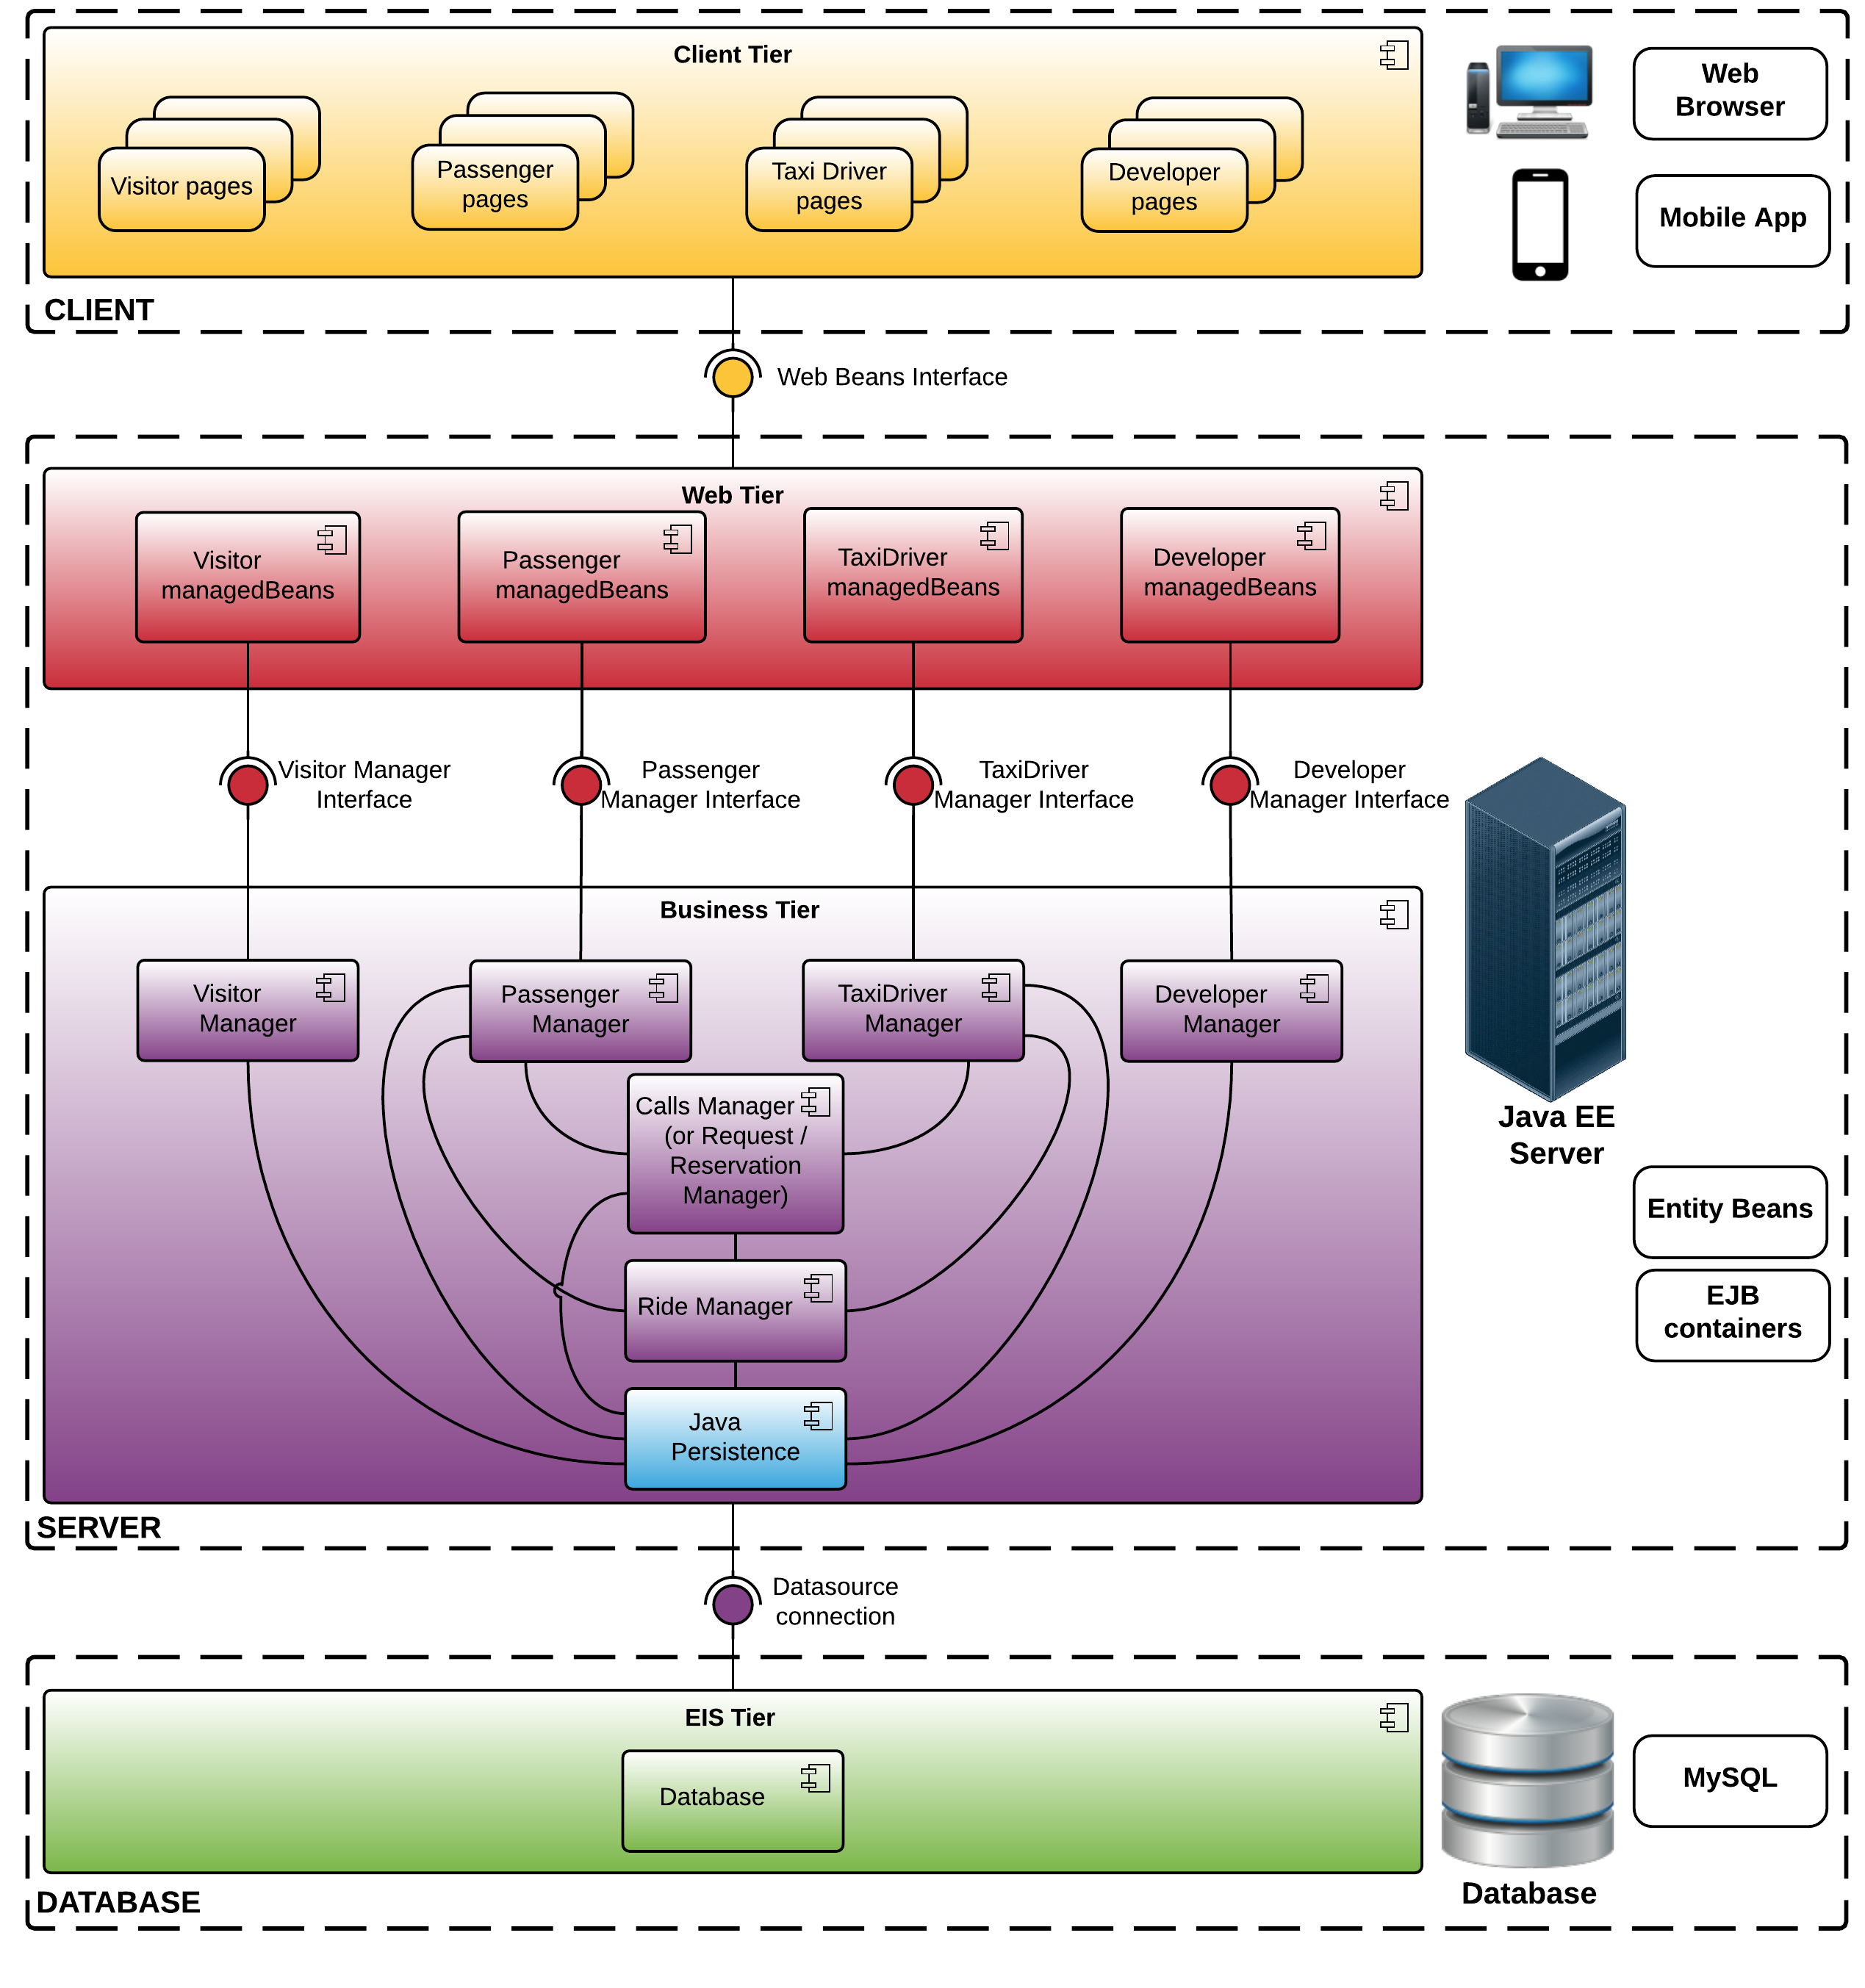
\includegraphics[width=\textwidth]{cpt/img/HighLevelComponentView}
\caption{High Level Components view and their interaction}
\label{fig:HLC}
\end{figure}
\clearpage

\section{Component View}
\subsection{Client Component}
The first component inside the system is the Client component which is responsible of translating user actions and presenting the output of tasks and results into something the user can understand. This component present different interfaces that allows each user to visualize the right pages. Each interface is a subcomponent of the Client components and contains different pages, so different users can visualize different contents with respect to their type.

\begin{figure}[htbp]
\centering
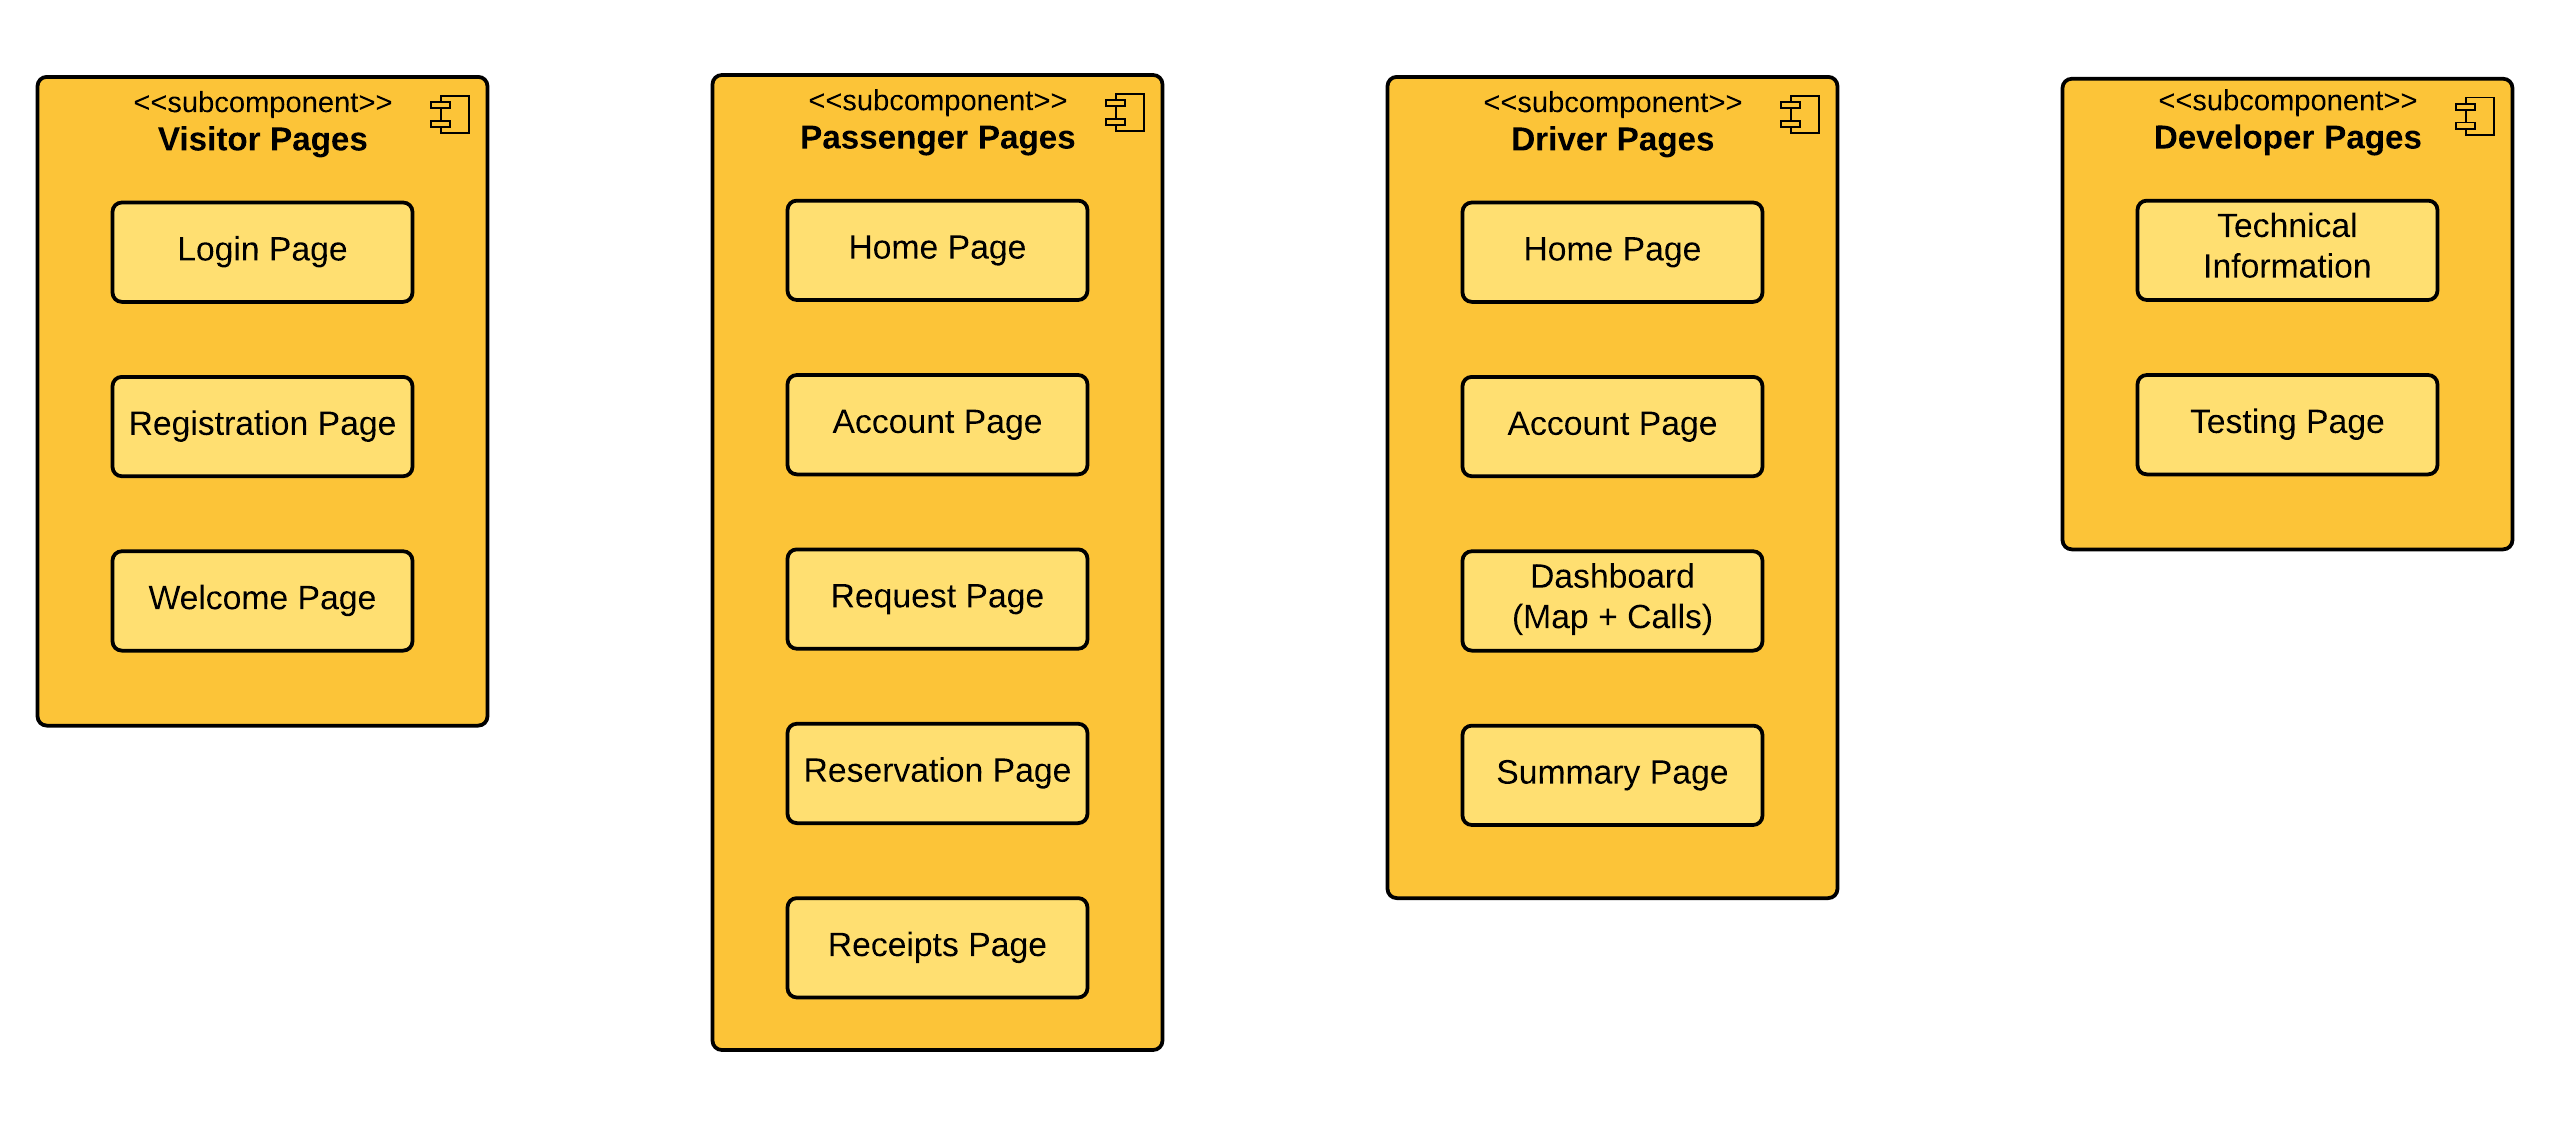
\includegraphics[width=\textwidth]{cpt/img/ClientInterfaces}
\caption{Client subcomponents}
\end{figure}
\clearpage

\subsection{Web Component}
The Web component generates dynamic web pages containing XHTML.
Web components are developed with Java Server Faces technology, which is a user
interface component framework for web applications.

\begin{figure}[htbp]
\centering
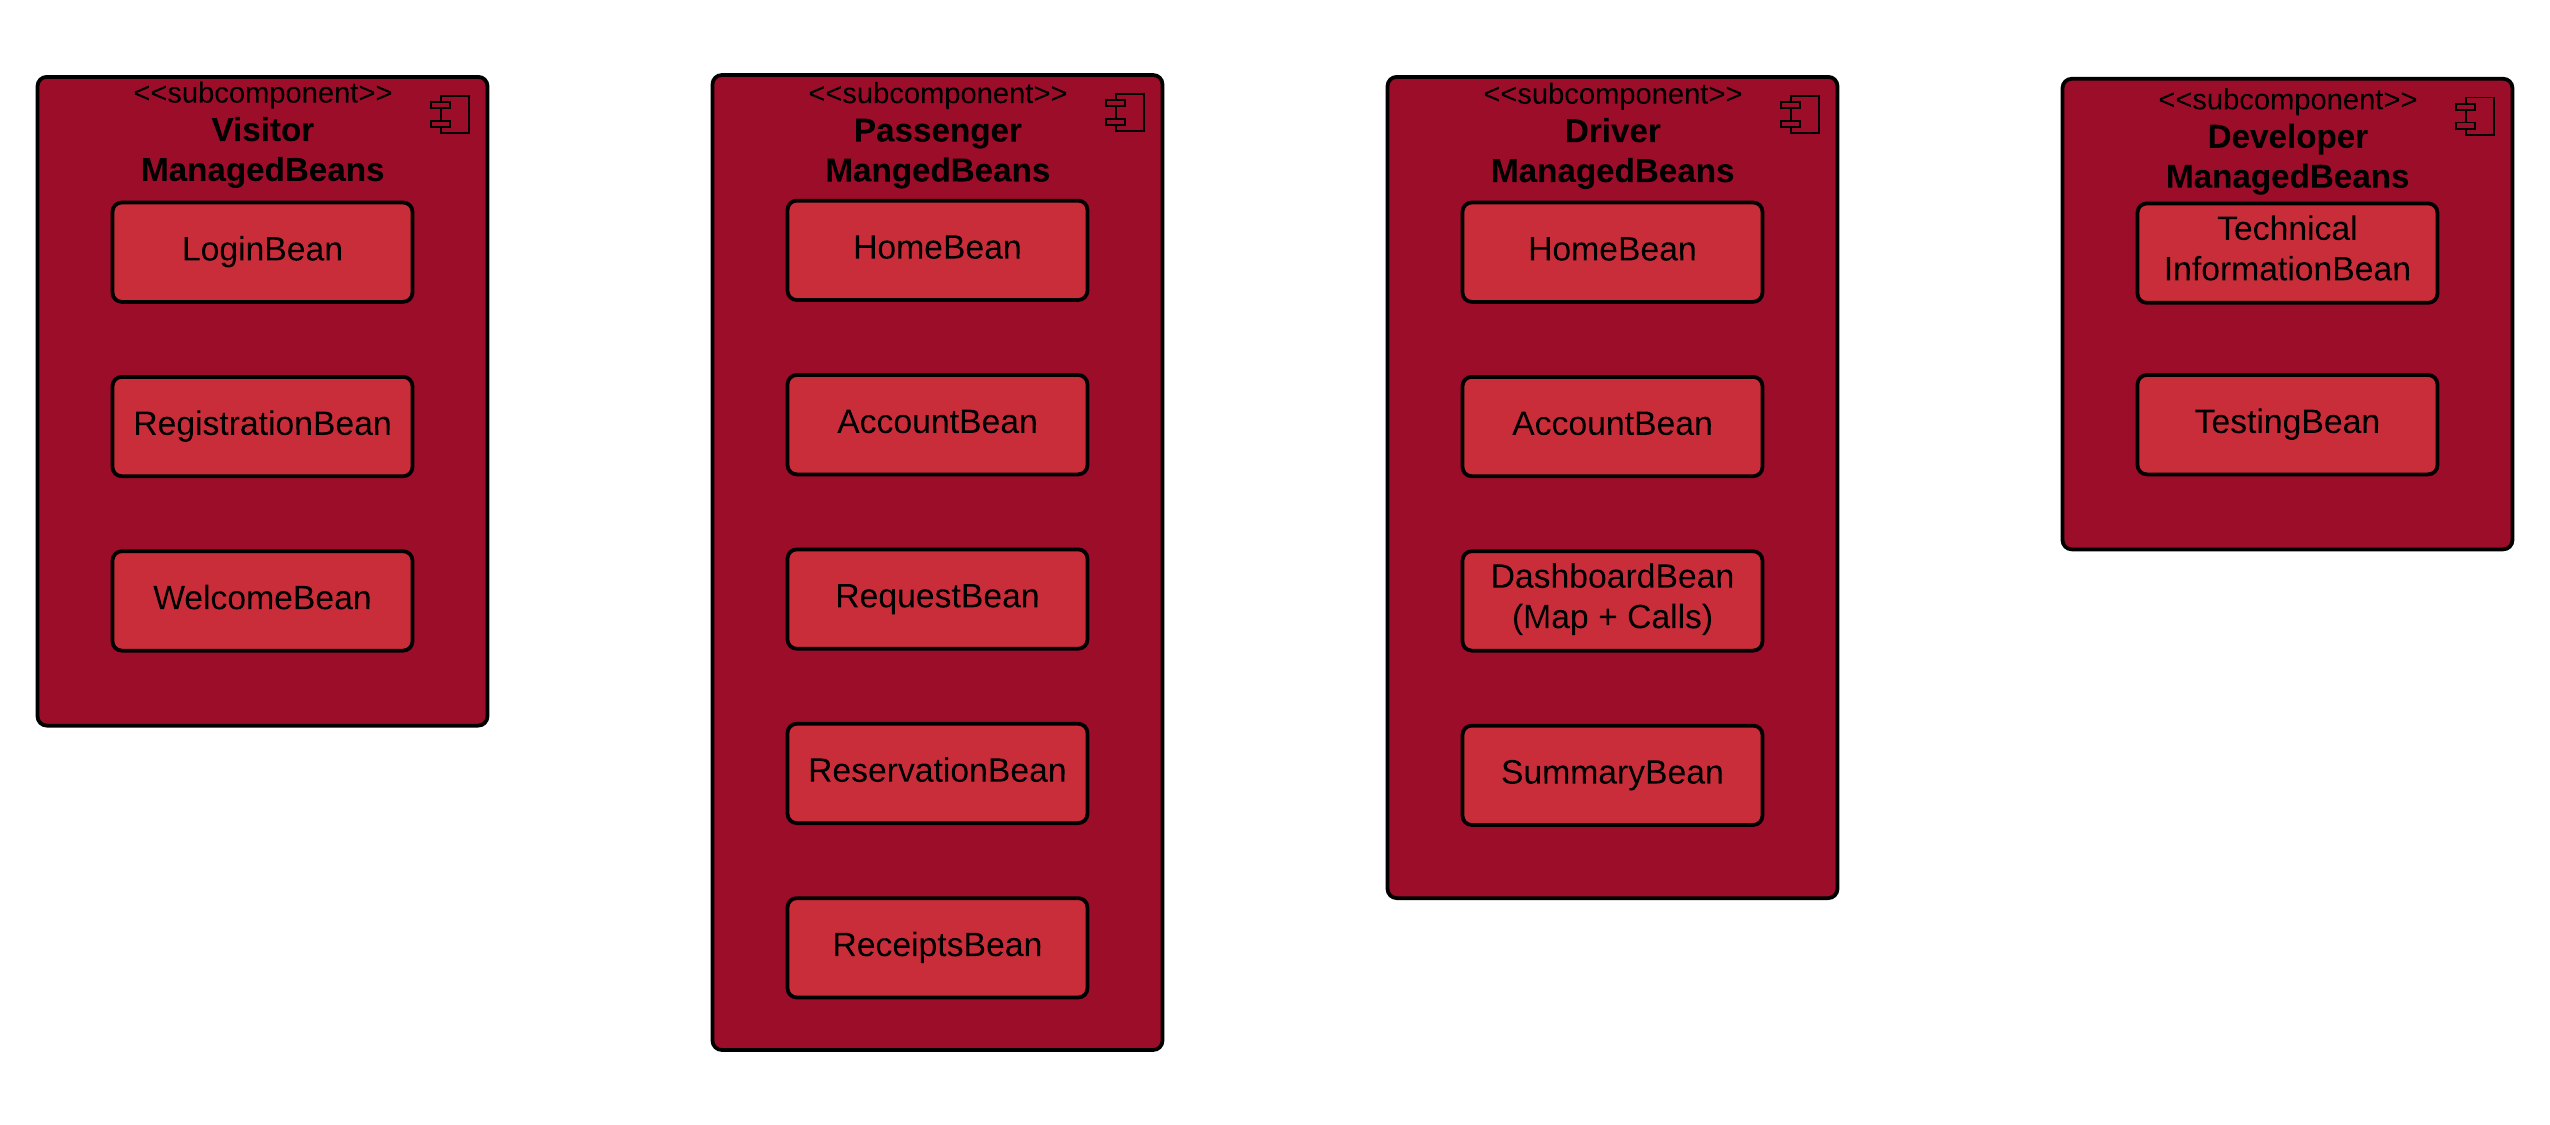
\includegraphics[width=\textwidth]{cpt/img/WebInterfaces}
\caption{Web subcomponents}
\end{figure}
\clearpage

\subsection{Business Logic Component}
Another component of the system is the Business Logic component, which coordinates the application, processes commands, makes logical decisions and evaluations, and performs calculations. It also moves and processes data between the Client and the Java Persistence, which holds the information of the system data model, and is in charge of storing and retrieving information from a database.
More in detail:
\begin{itemize}
	\item Visitor Manager $\rightarrow$ Offers functionalities to:
	\begin{itemize}
		\item Check the validity and correctness of the information provided by the user 
		\item Create new users and save them into the system;
		\item Check if the Login is valid and authenticate users;
		\item Trigger the right user manager depending on the type of user that has logged in.
	\end{itemize}
	\item Passenger Manager $\rightarrow$ Manages the passenger requests (taxi requests, reservations), the passenger profile and his status.
	\item Taxi Driver Manager $\rightarrow$ Manages all the operations made by taxi drivers, like accepting or rejecting incoming calls or ending rides
	\item Developer Manager $\rightarrow$ Manage all the operations made by developers (add new features)
	\item Ride Manager $\rightarrow$ Offers functionalities to:
	\begin{itemize}
		\item Create and manage the route for the ride;
		\item Keep track of the passengers and the driver involved in the ride, and all the information: duration, distance, fee, route for the entire ride and for each passenger.
	\end{itemize}
	\item Call Manager $\rightarrow$ Manages all the passenger?s requests/reservations, the taxi queue for every area and the matching for show rides.
\end{itemize}

\begin{figure}[htbp]
\centering
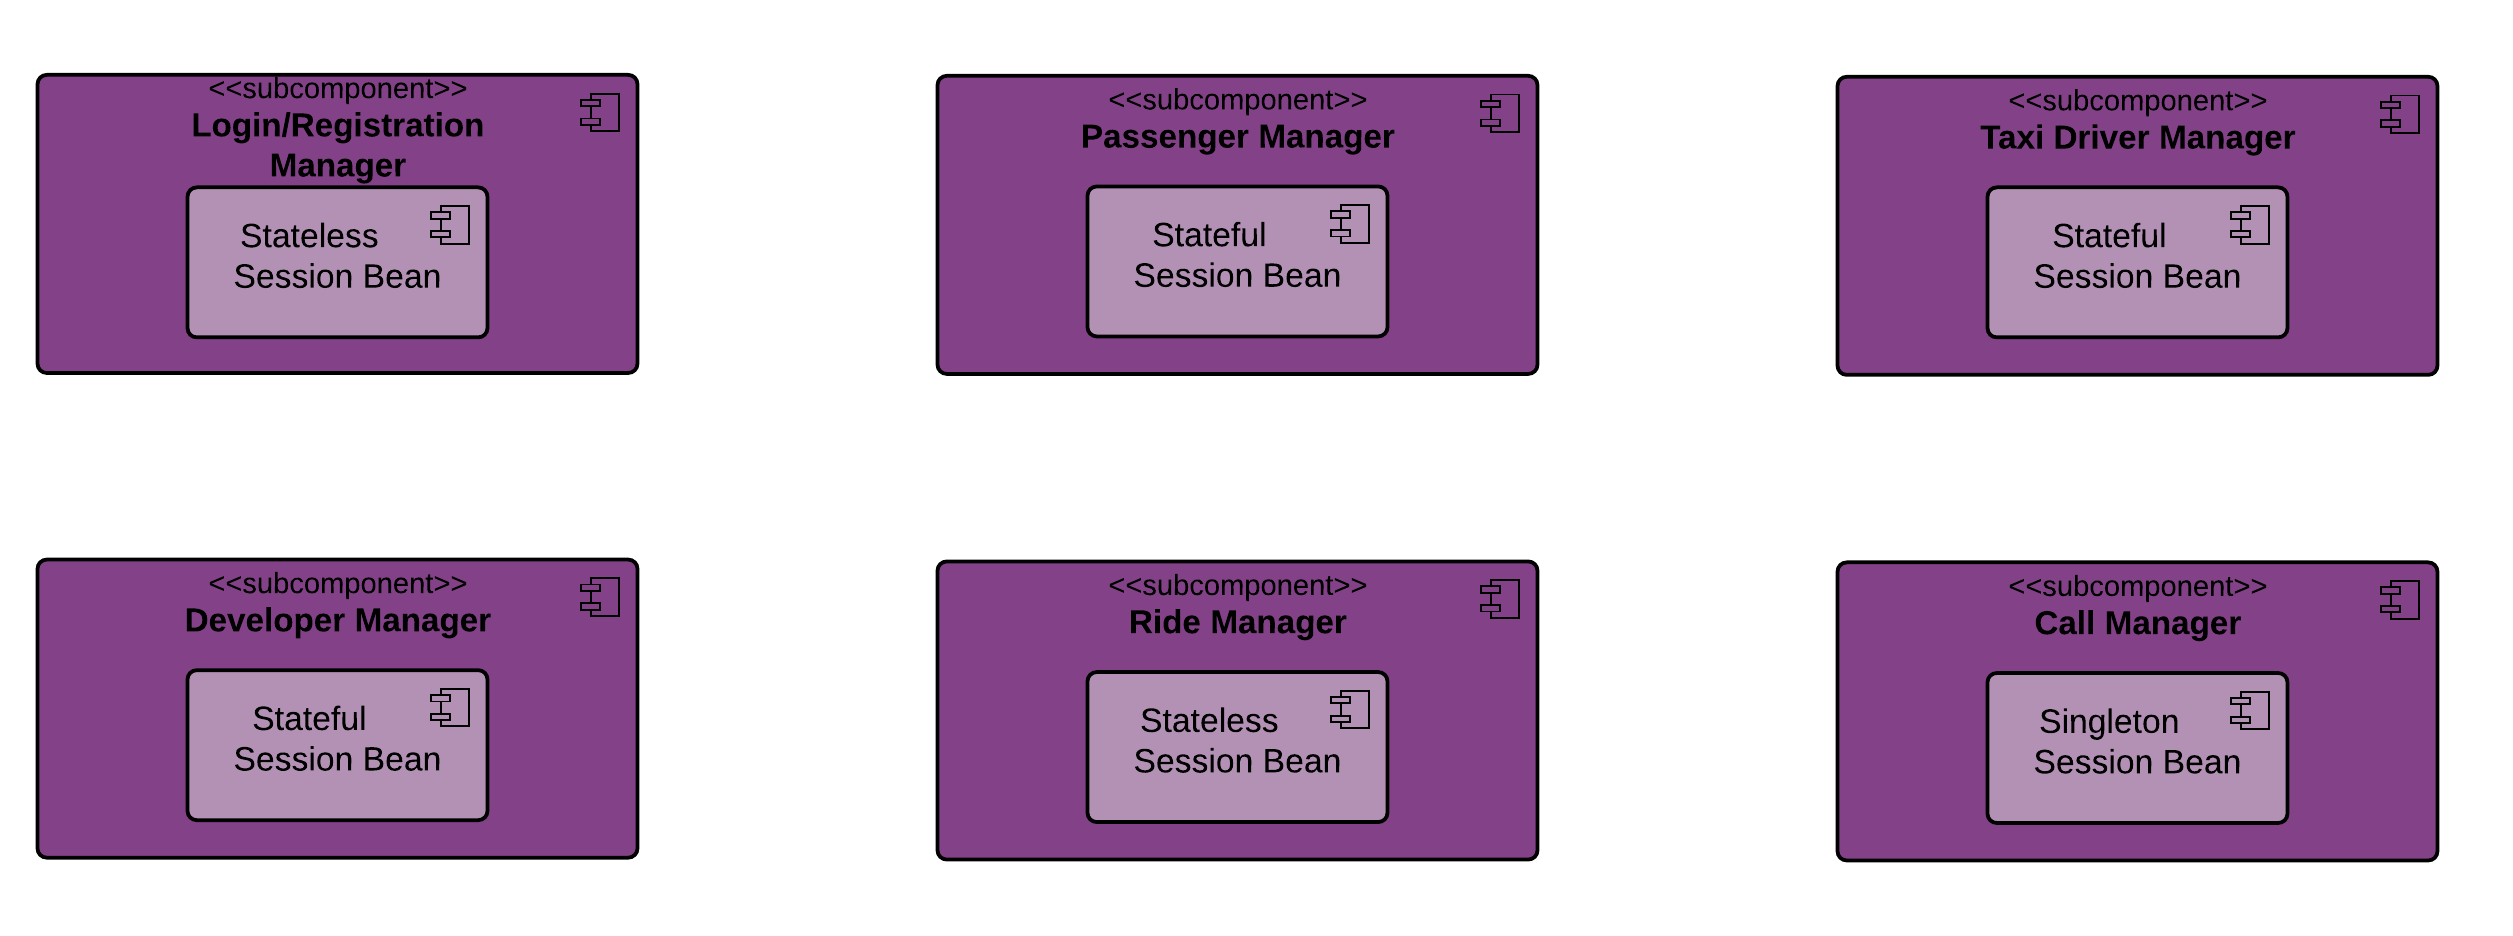
\includegraphics[width=\textwidth]{cpt/img/ServerInterfaces}
\caption{Business Logic subcomponents}
\end{figure}
\clearpage

\subsection{Database Component}
The last component of the system is represented by the Database that contains all the data that are interesting for this application.

\begin{figure}[htbp]
\centering
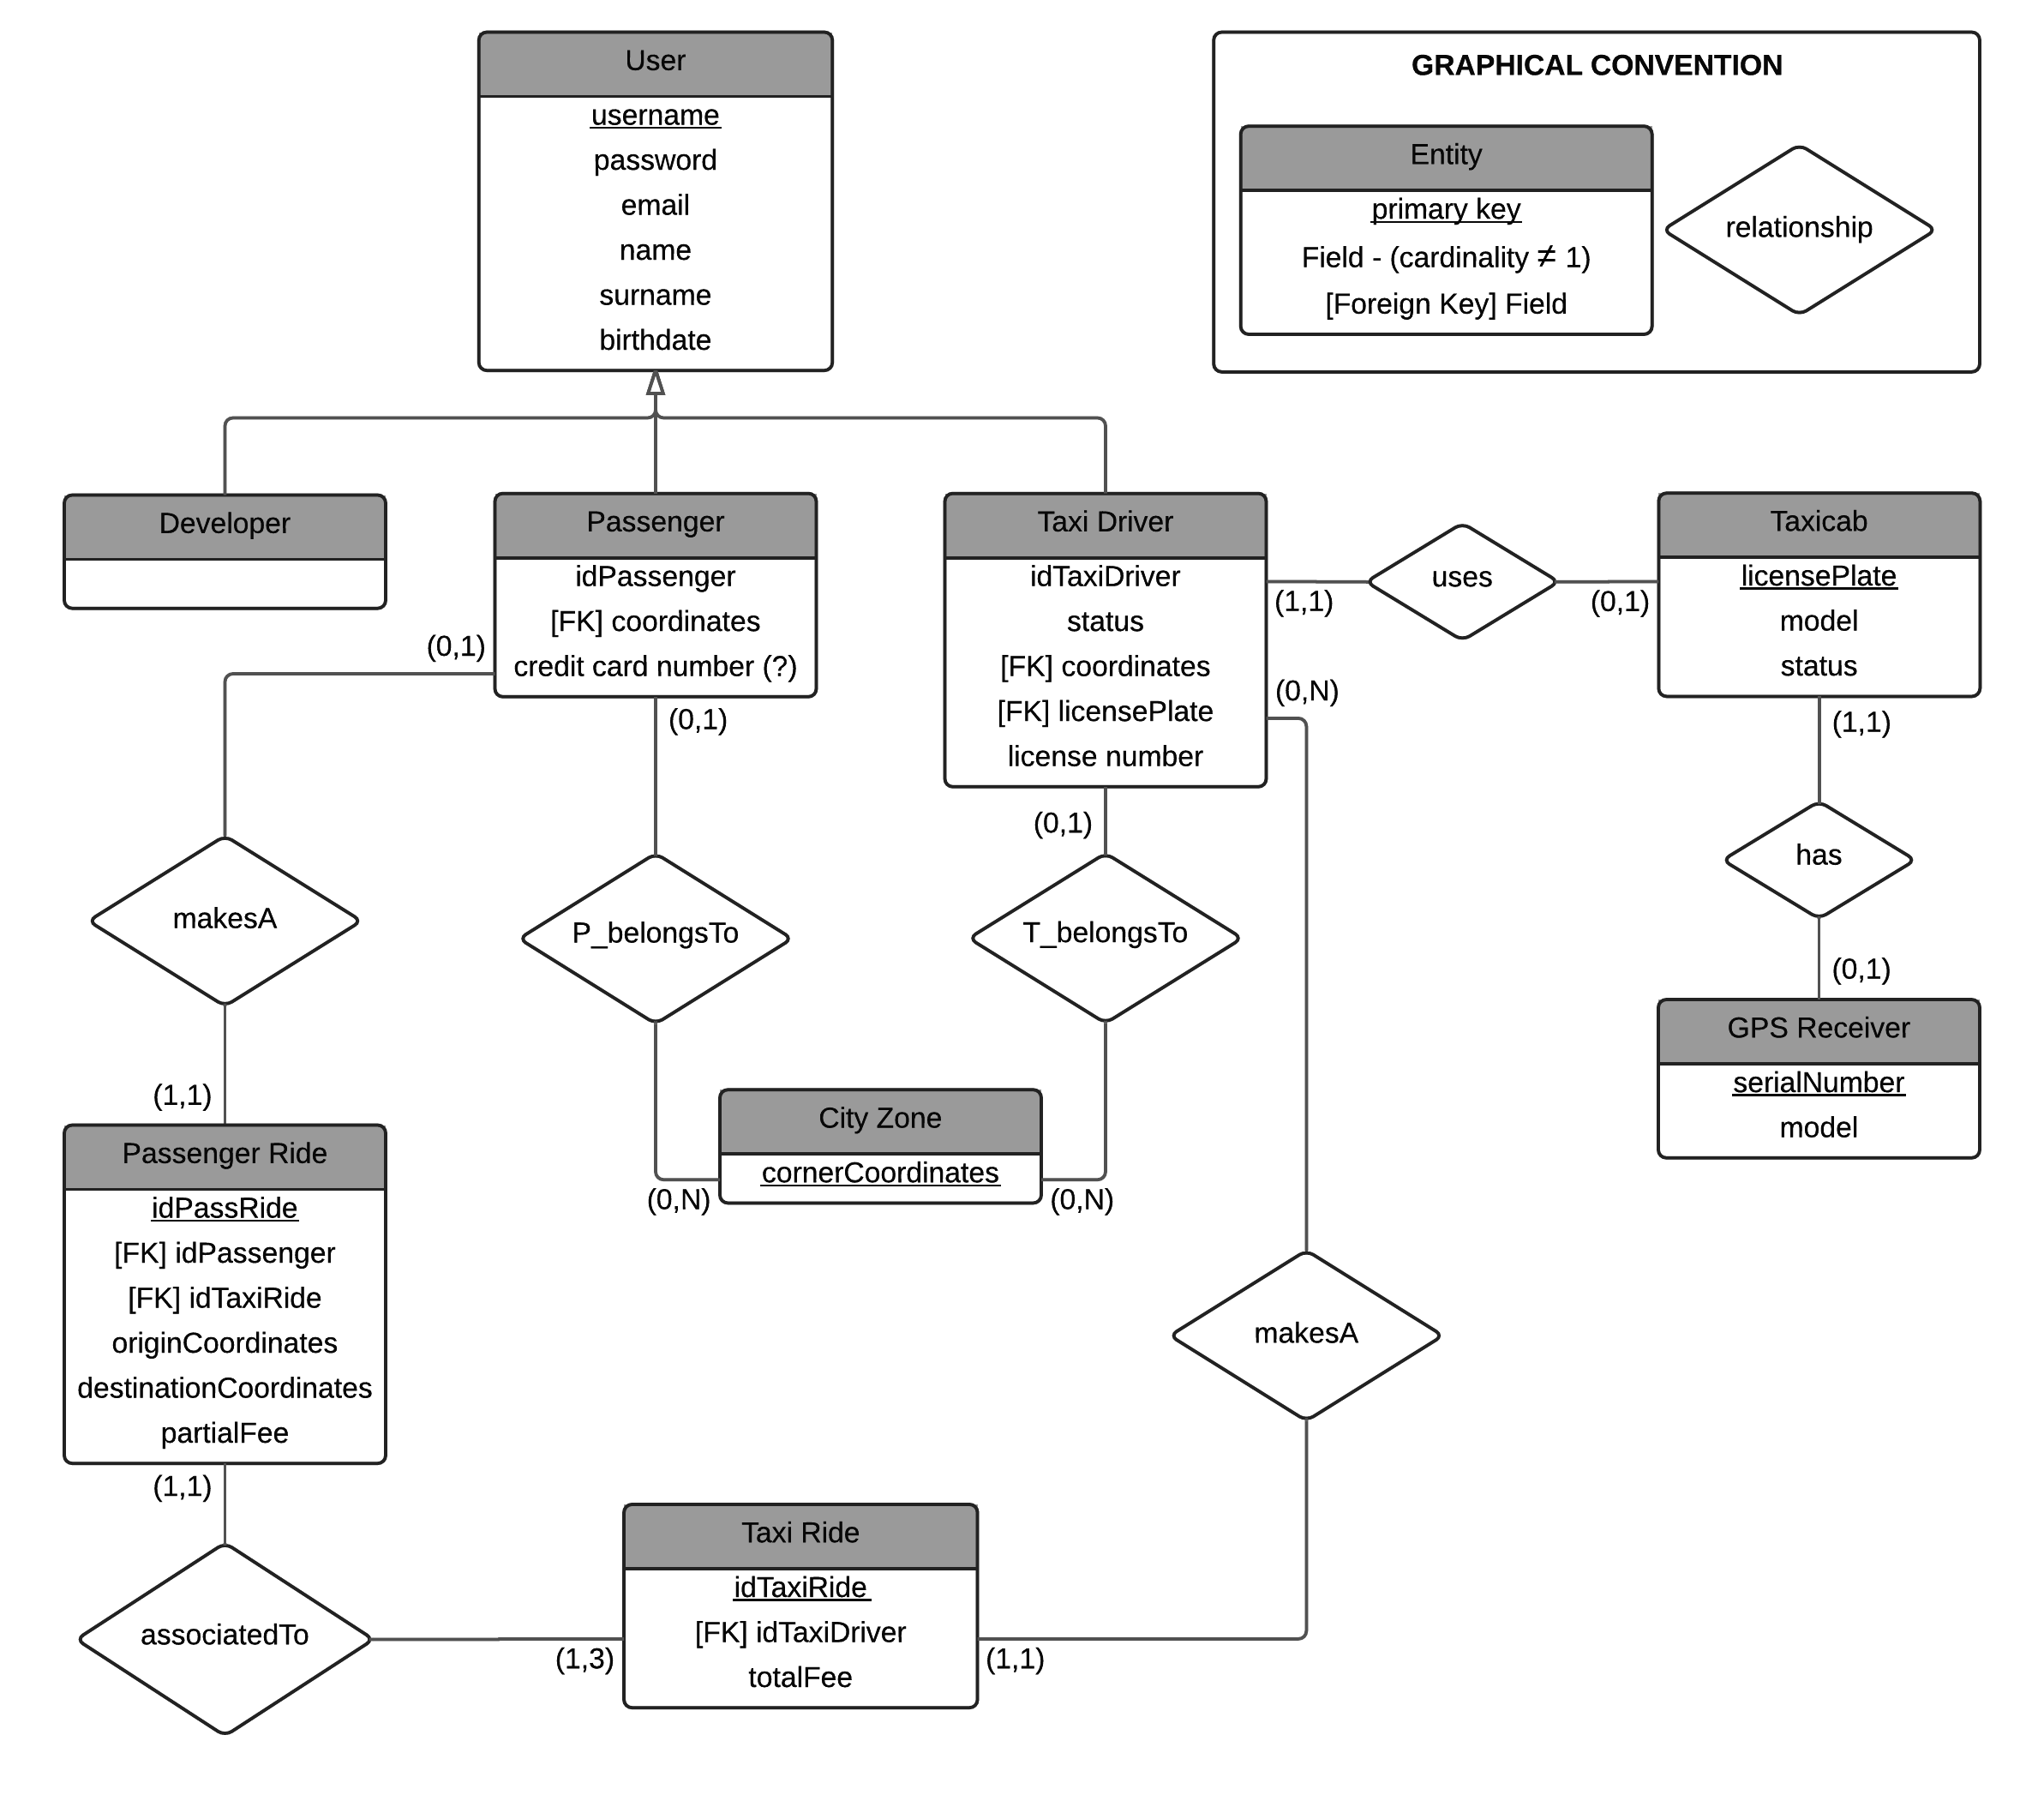
\includegraphics[width=\textwidth]{cpt/img/Database}
\caption{Database ER Diagram}
\end{figure}
\clearpage

\section{Deployment View}
The diagram in Figure \ref{fig:Deploy} shows the deployment view of the software product.

\begin{figure}[htbp]
\centering
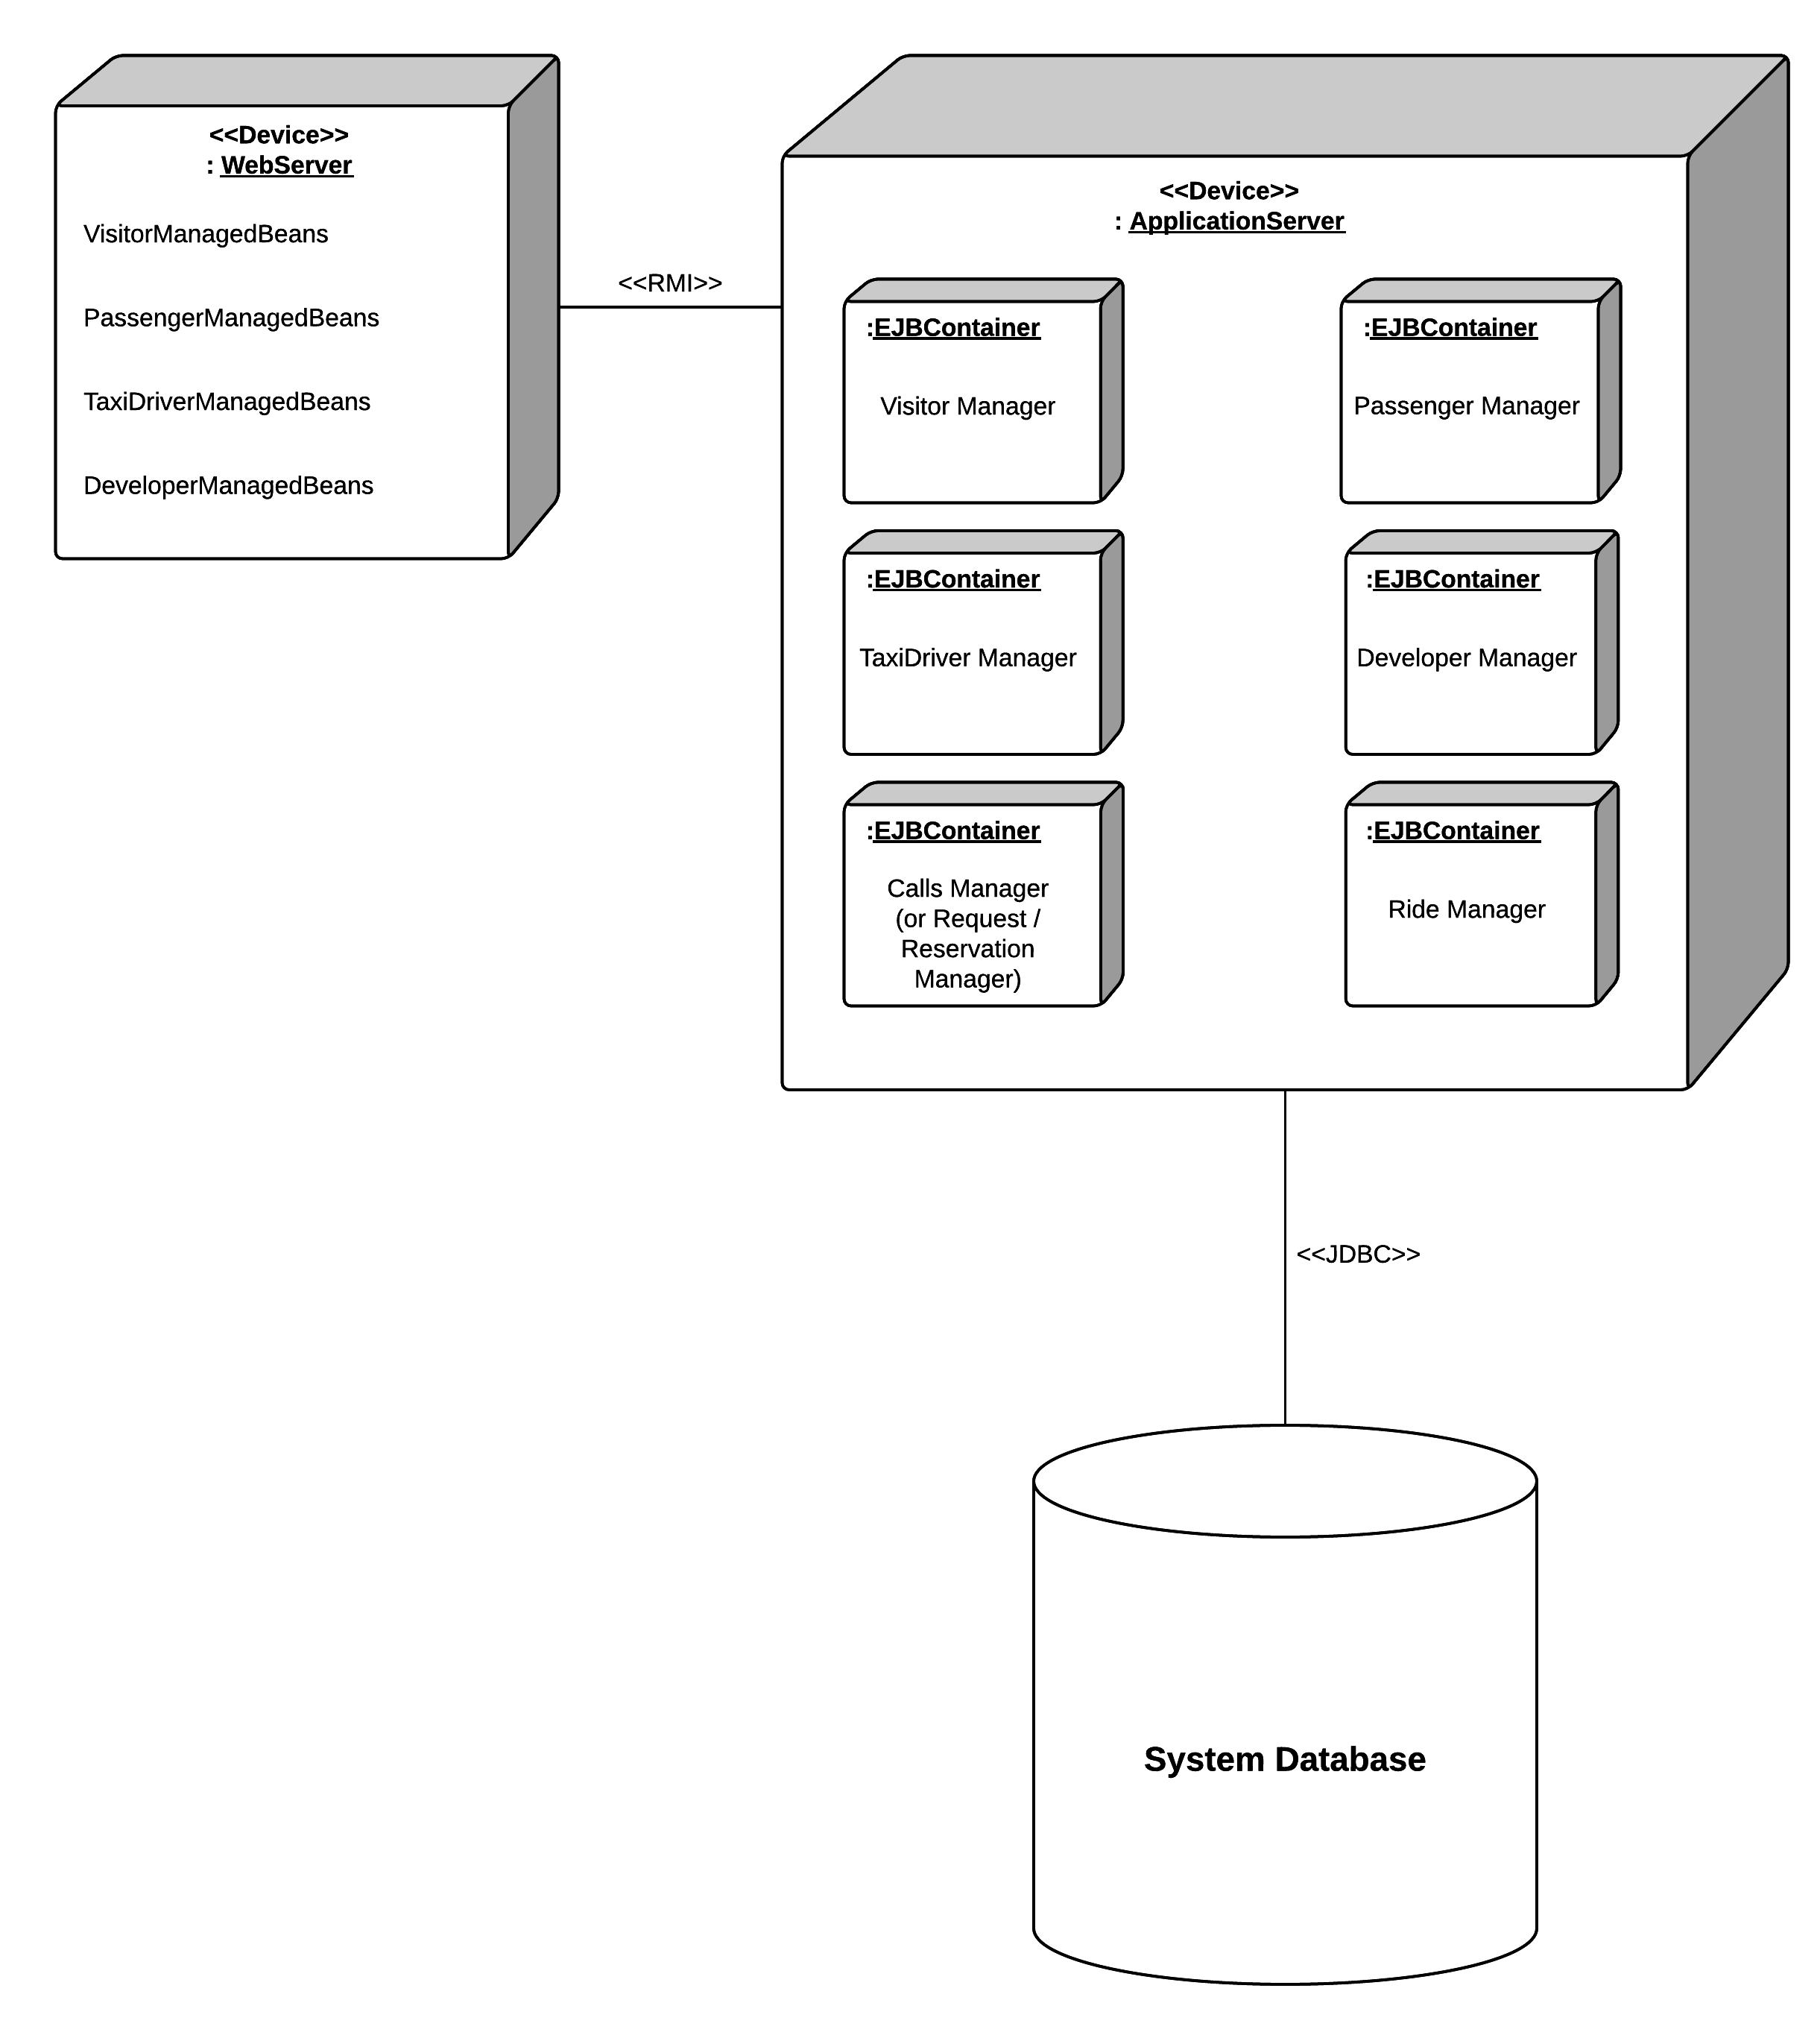
\includegraphics[width=\textwidth]{cpt/img/RuntimeDeploymentView}
\caption{Deployment view}
\label{fig:Deploy}
\end{figure}
\clearpage

\section{Runtime View}
The following diagrams describes the runtime view of MyTaxiService project describing the way components behave in order to accomplish the most important activities of the system. The software product that will be released can be deployed in any a JEE Application Server:

\begin{itemize}
	\item This diagram represent the components that are interested in the taxi request and reservation activities, and their interaction.
	\begin{figure}[htbp]
	\centering
	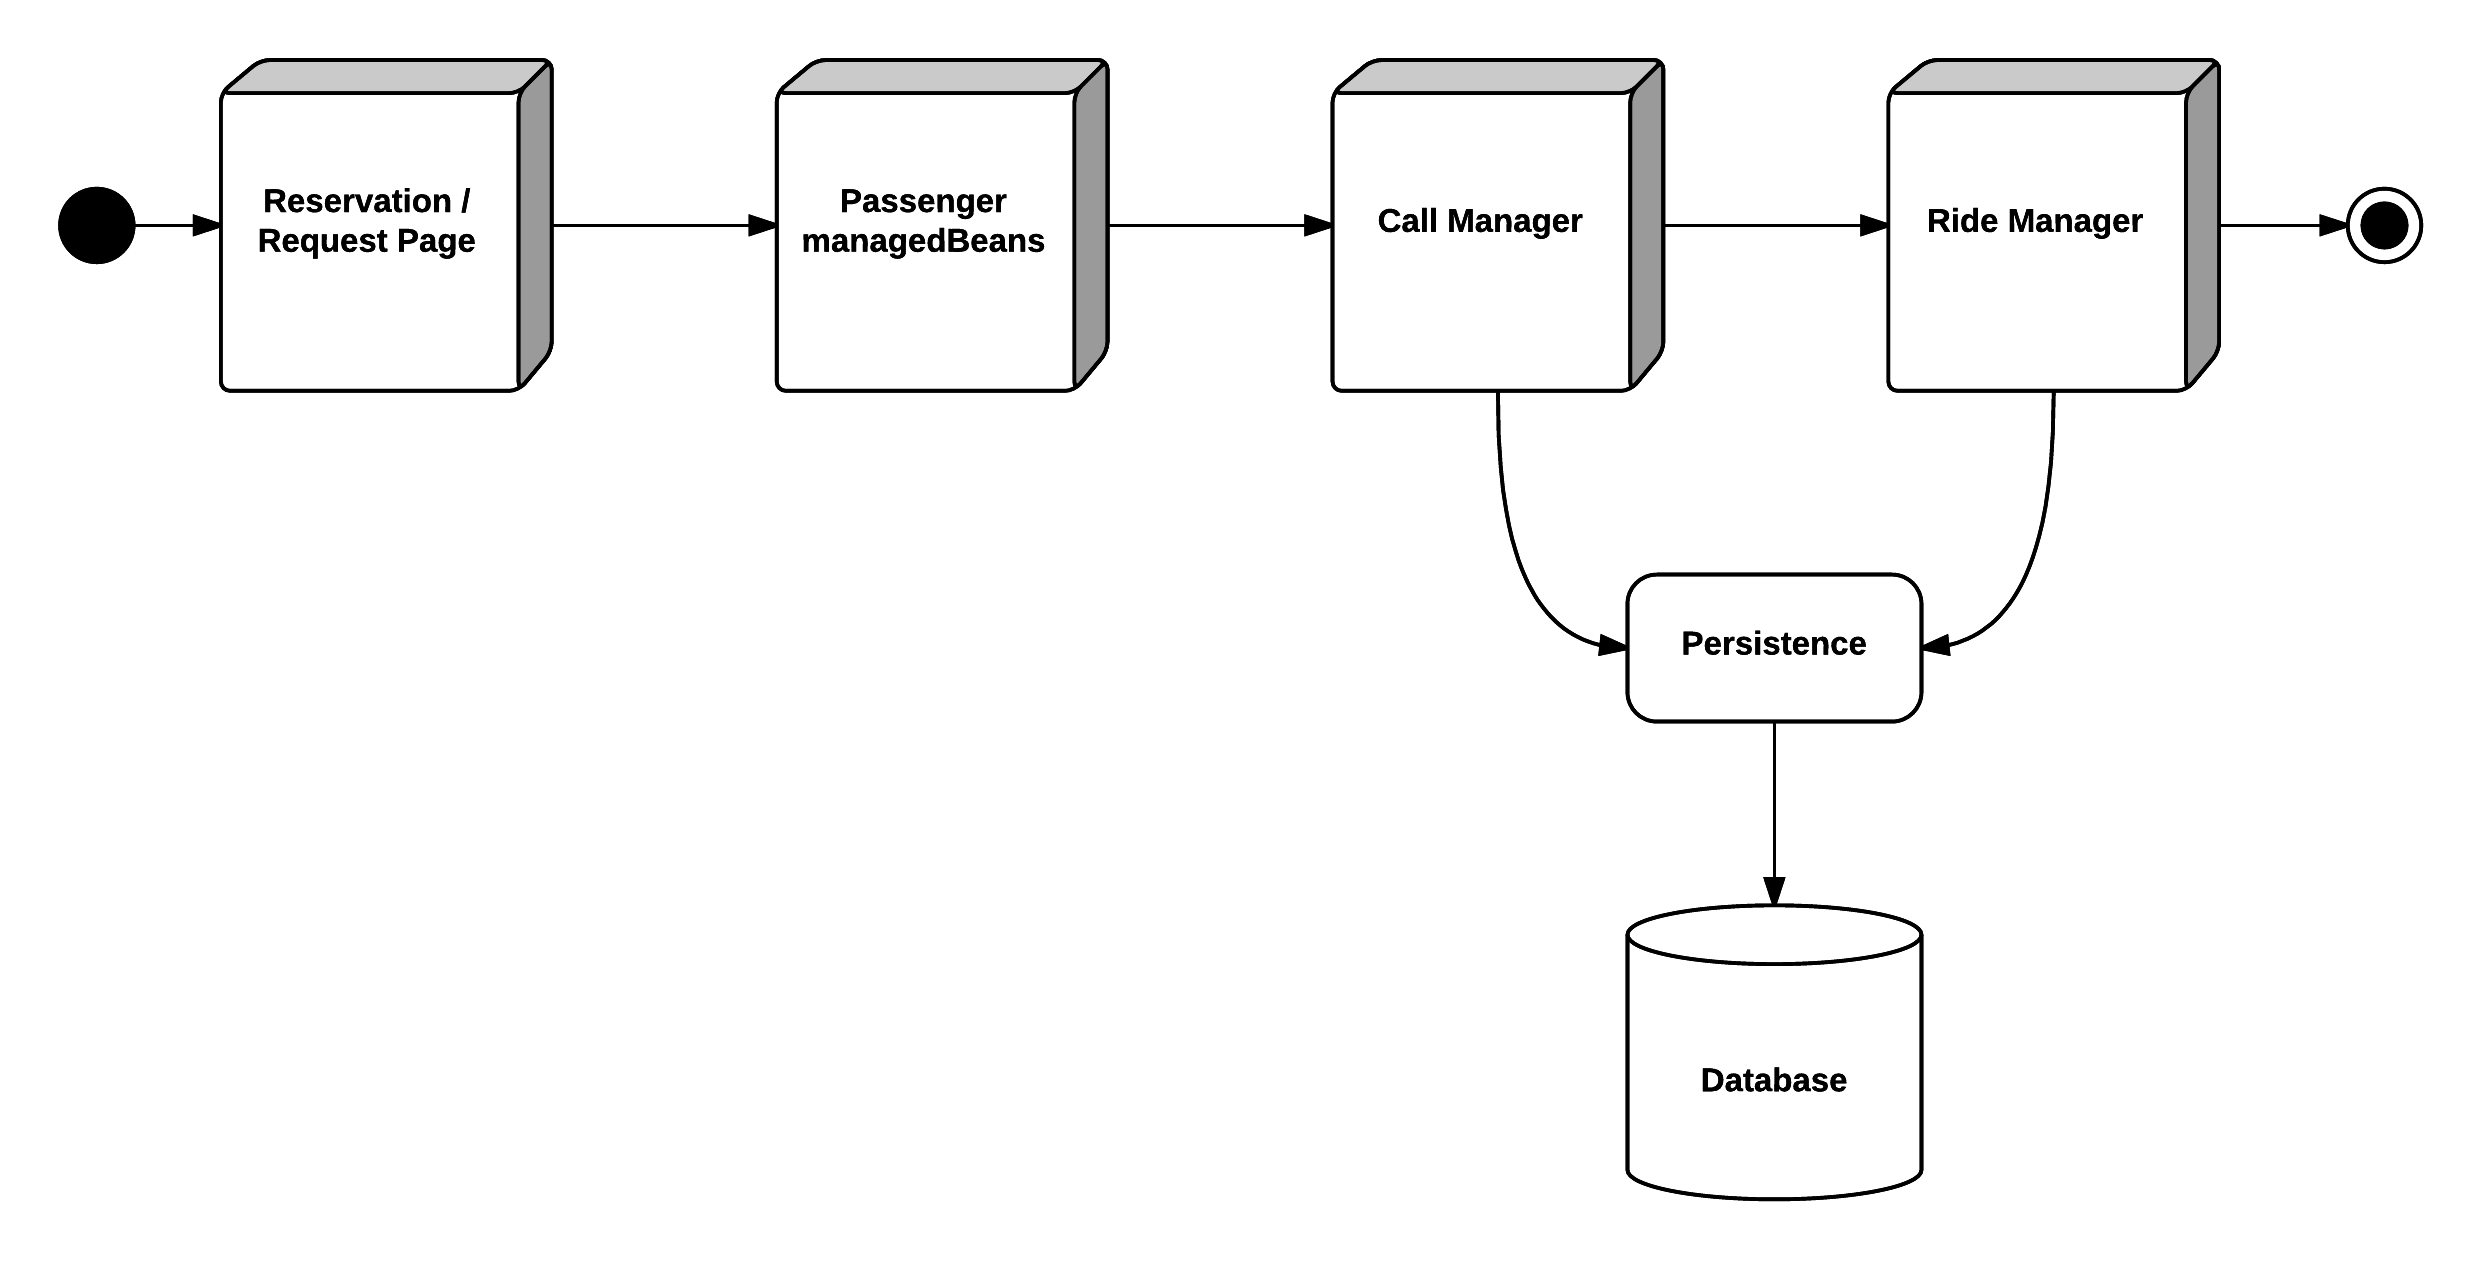
\includegraphics[width=\textwidth]{cpt/img/RuntimeReqResView}
	\caption{Runtime Taxi Request and Reservation}
	\end{figure}
	\clearpage
	
	\item This diagram represent the components that are interested in the getting receipts activity, and their interaction.
	\begin{figure}[htbp]
	\centering
	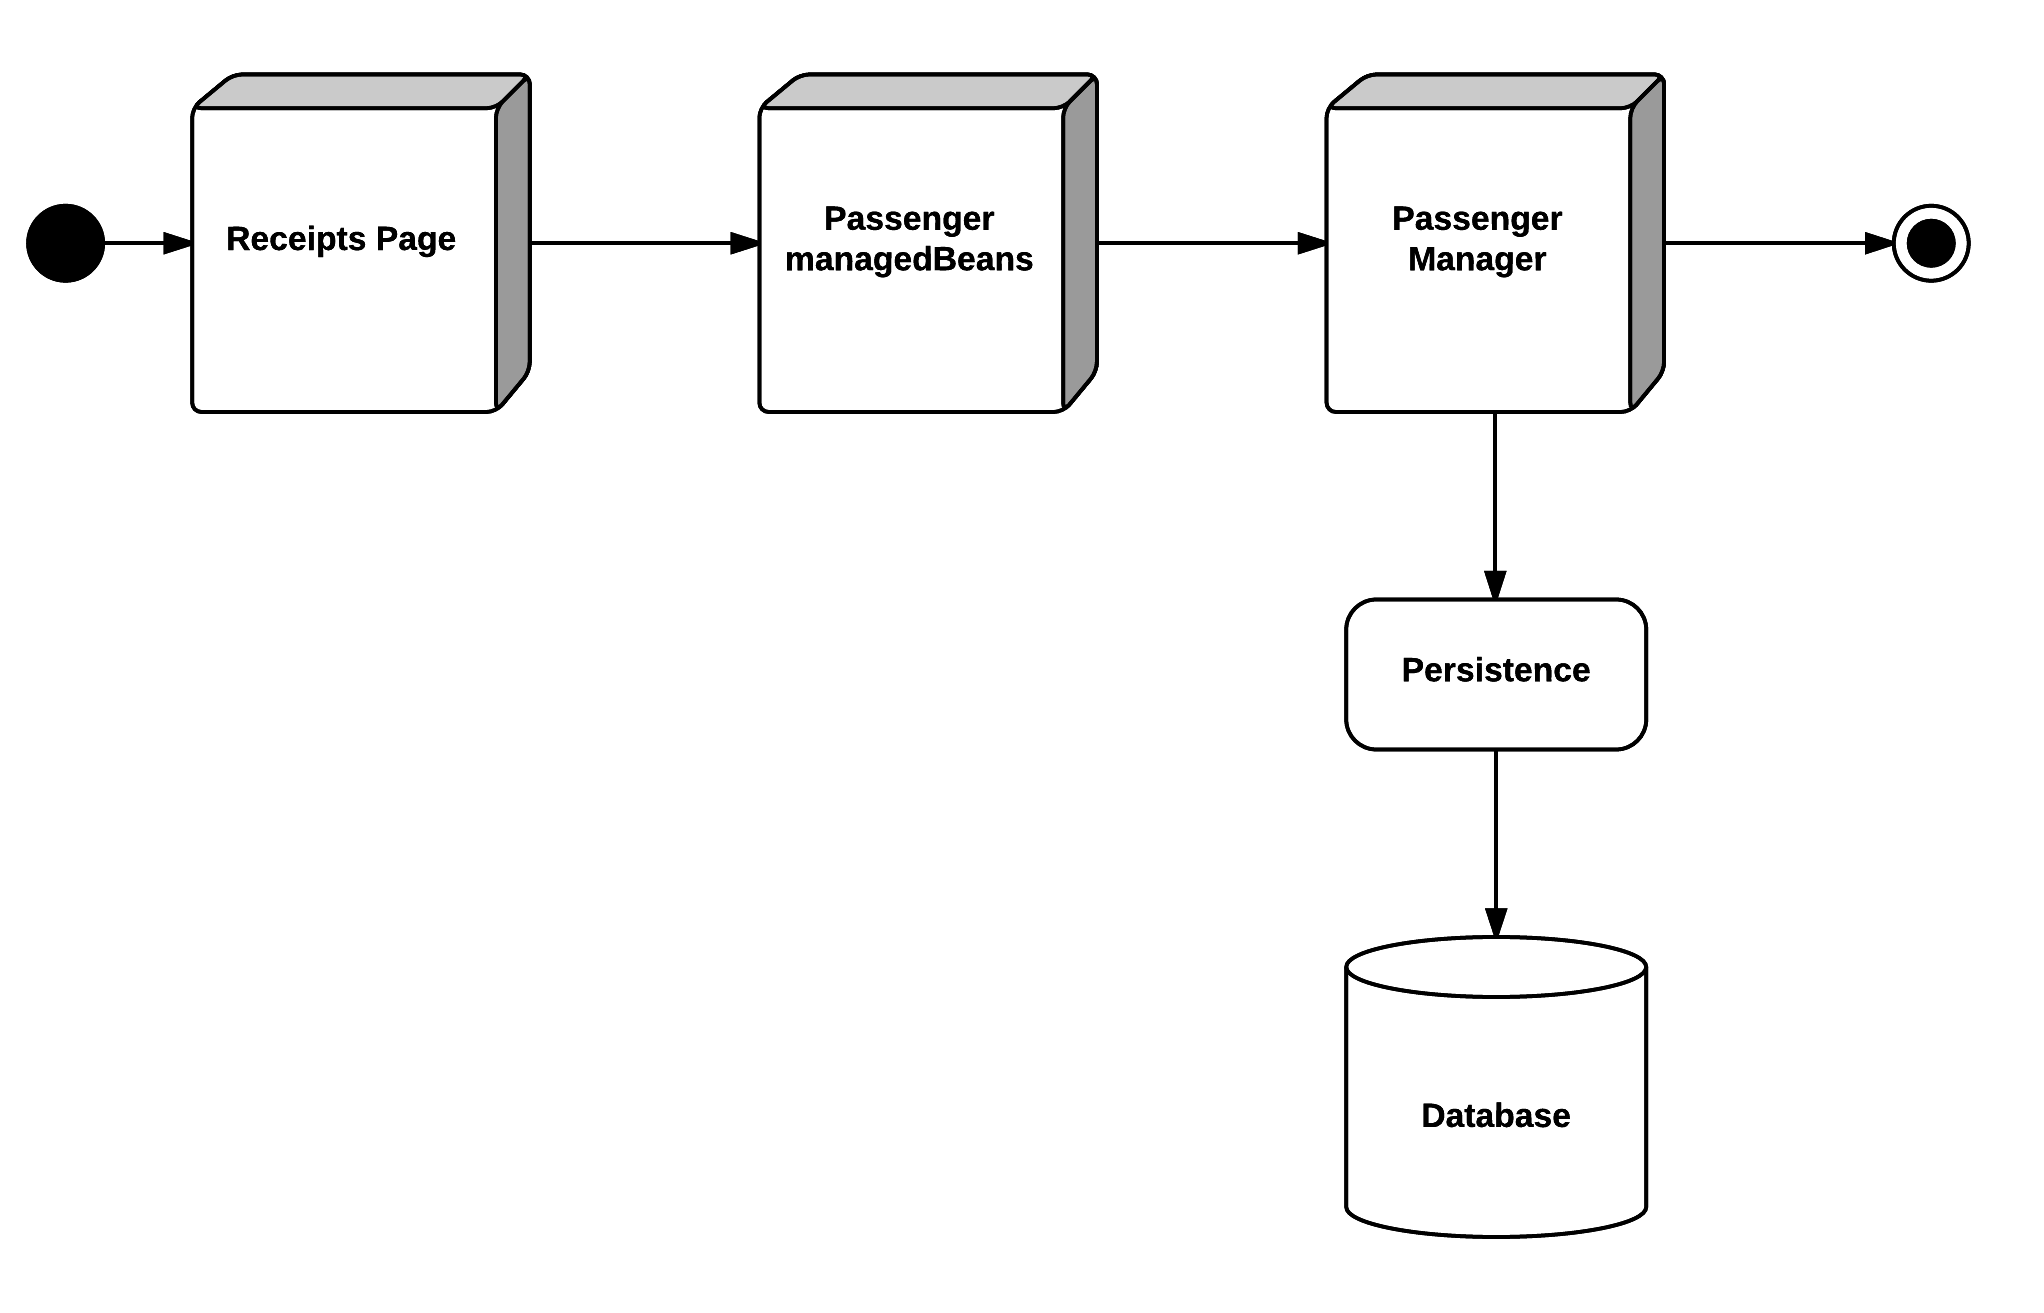
\includegraphics[width=\textwidth]{cpt/img/RuntimeReceiptsView}
	\caption{Runtime getting receipts}
	\end{figure}
	\clearpage
	
	\item This diagram represent the components that are interested in the modifying passenger's account activity, and their interaction.
	\begin{figure}[htbp]
	\centering
	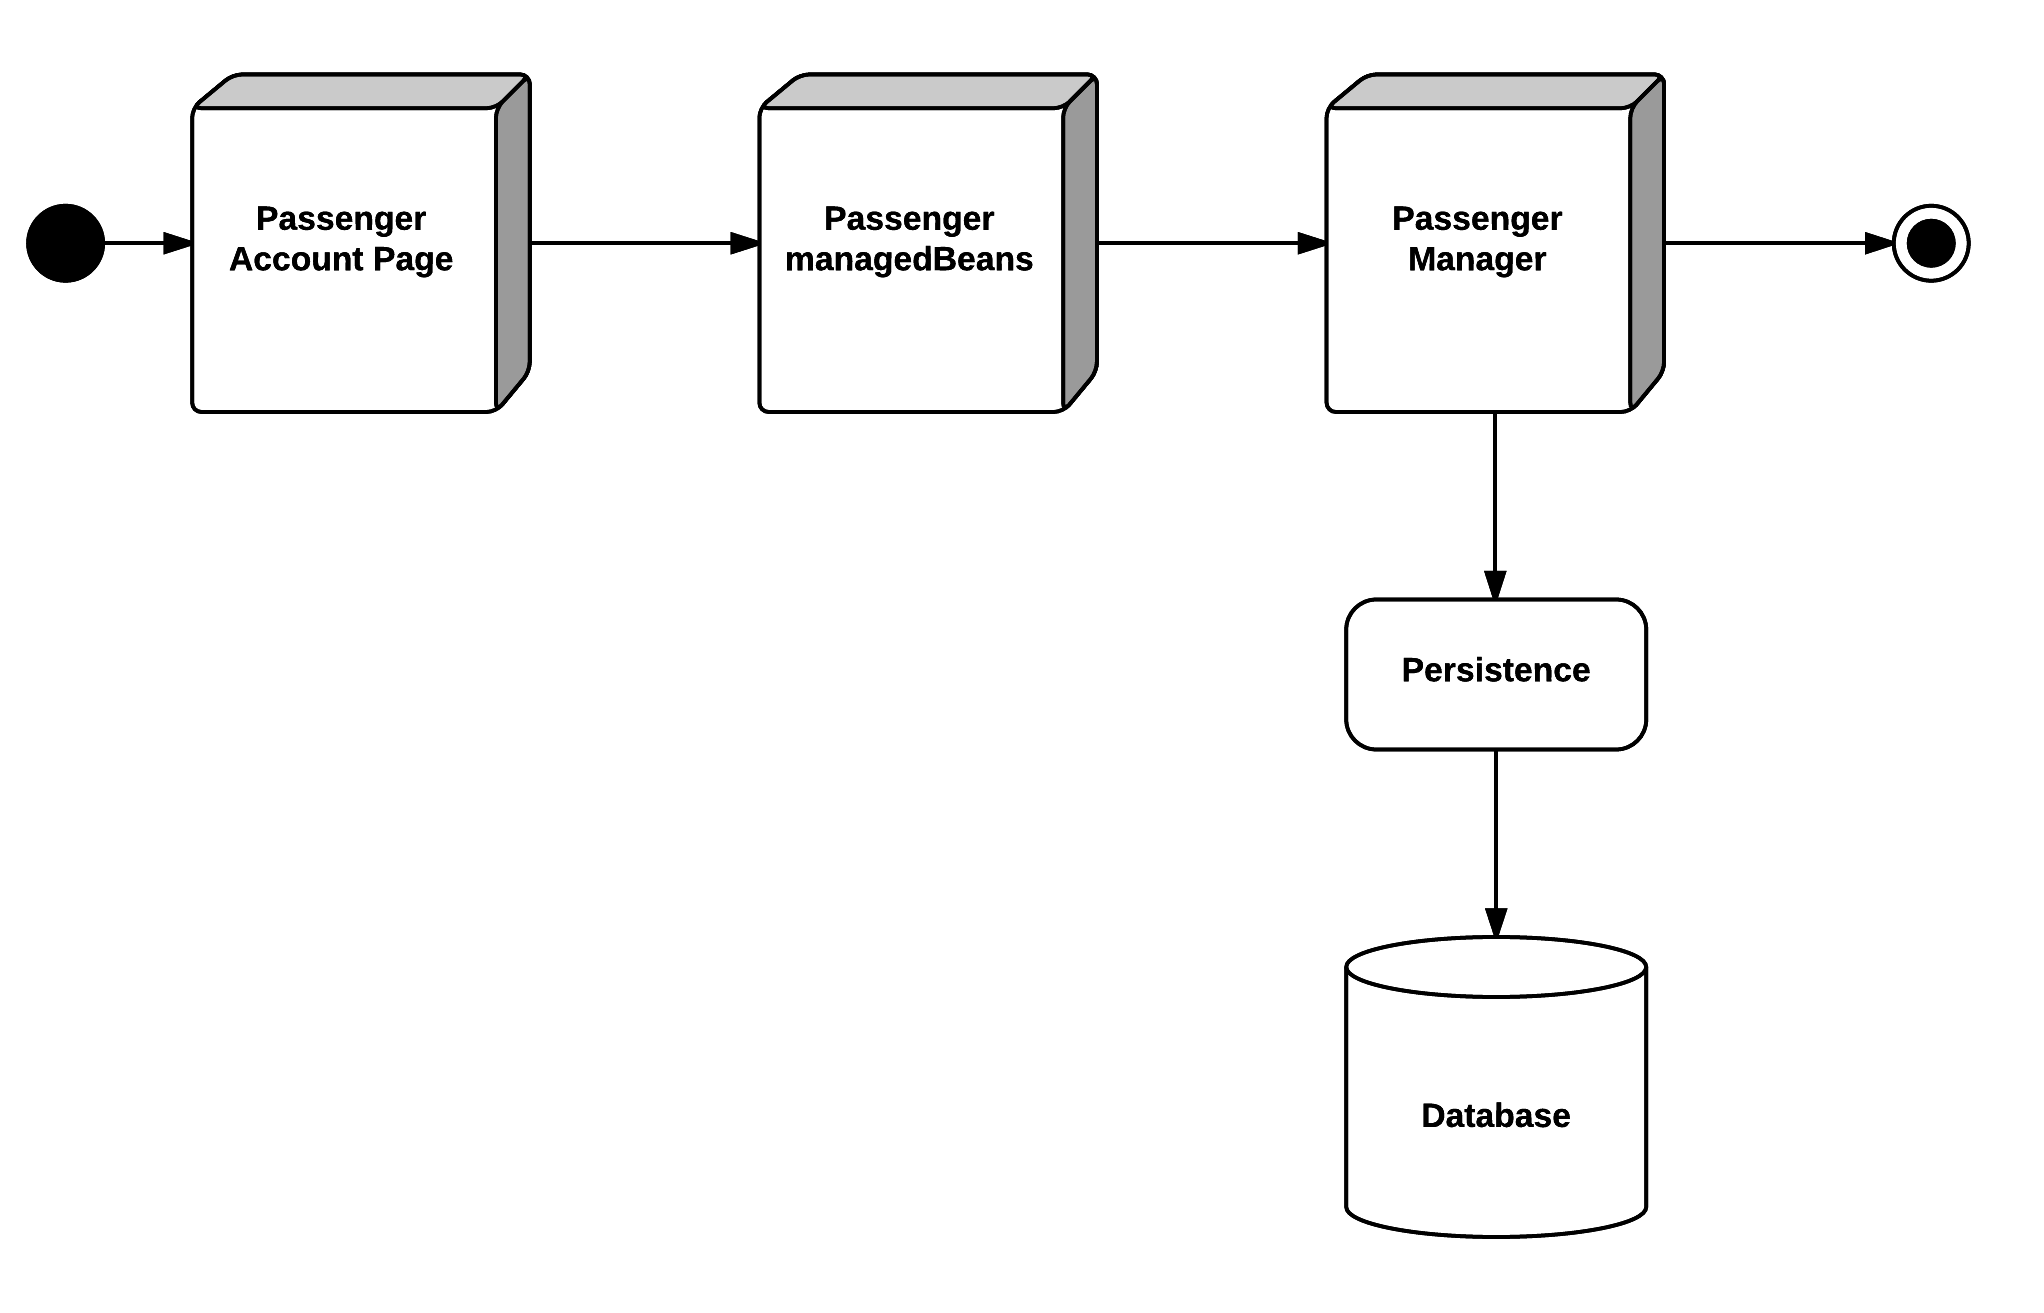
\includegraphics[width=\textwidth]{cpt/img/RuntimeModifyPageView}
	\caption{Runtime Modify Passenger's Account}
	\end{figure}
	\clearpage
	
	\item This diagram represent the components that are interested in the modifying taxi driver's account activity, and their interaction.
	\begin{figure}[htbp]
	\centering
	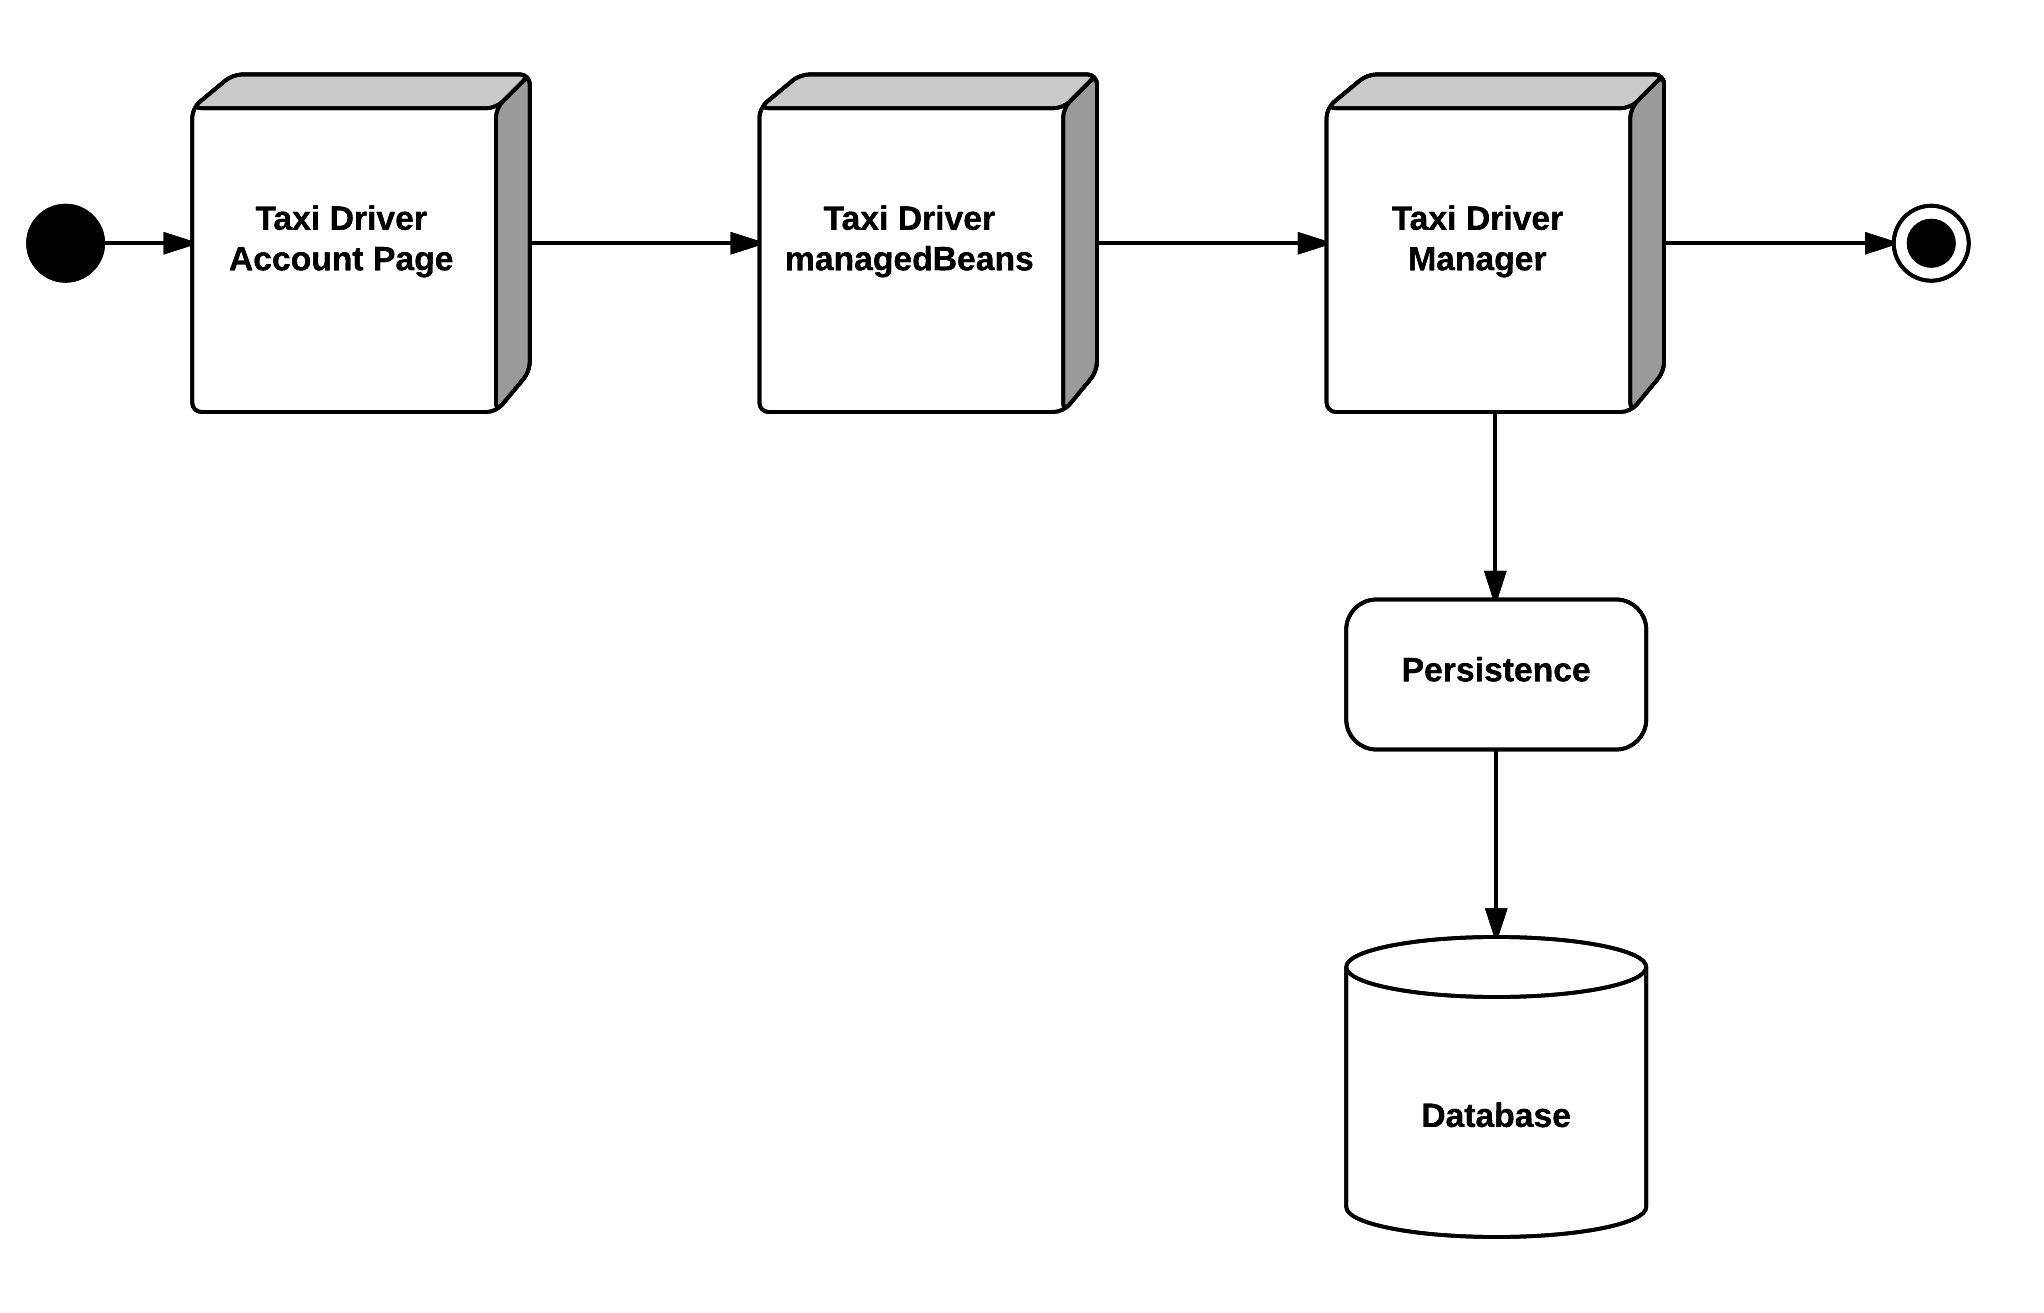
\includegraphics[width=\textwidth]{cpt/img/RuntimeModifyPageTaxidriverView}
	\caption{Runtime Modify Taxi Driver's Account}
	\end{figure}
	\clearpage
	
	\item This diagram represent the components that are interested in the login and registration activities, and their interaction.
	\begin{figure}[htbp]
	\centering
	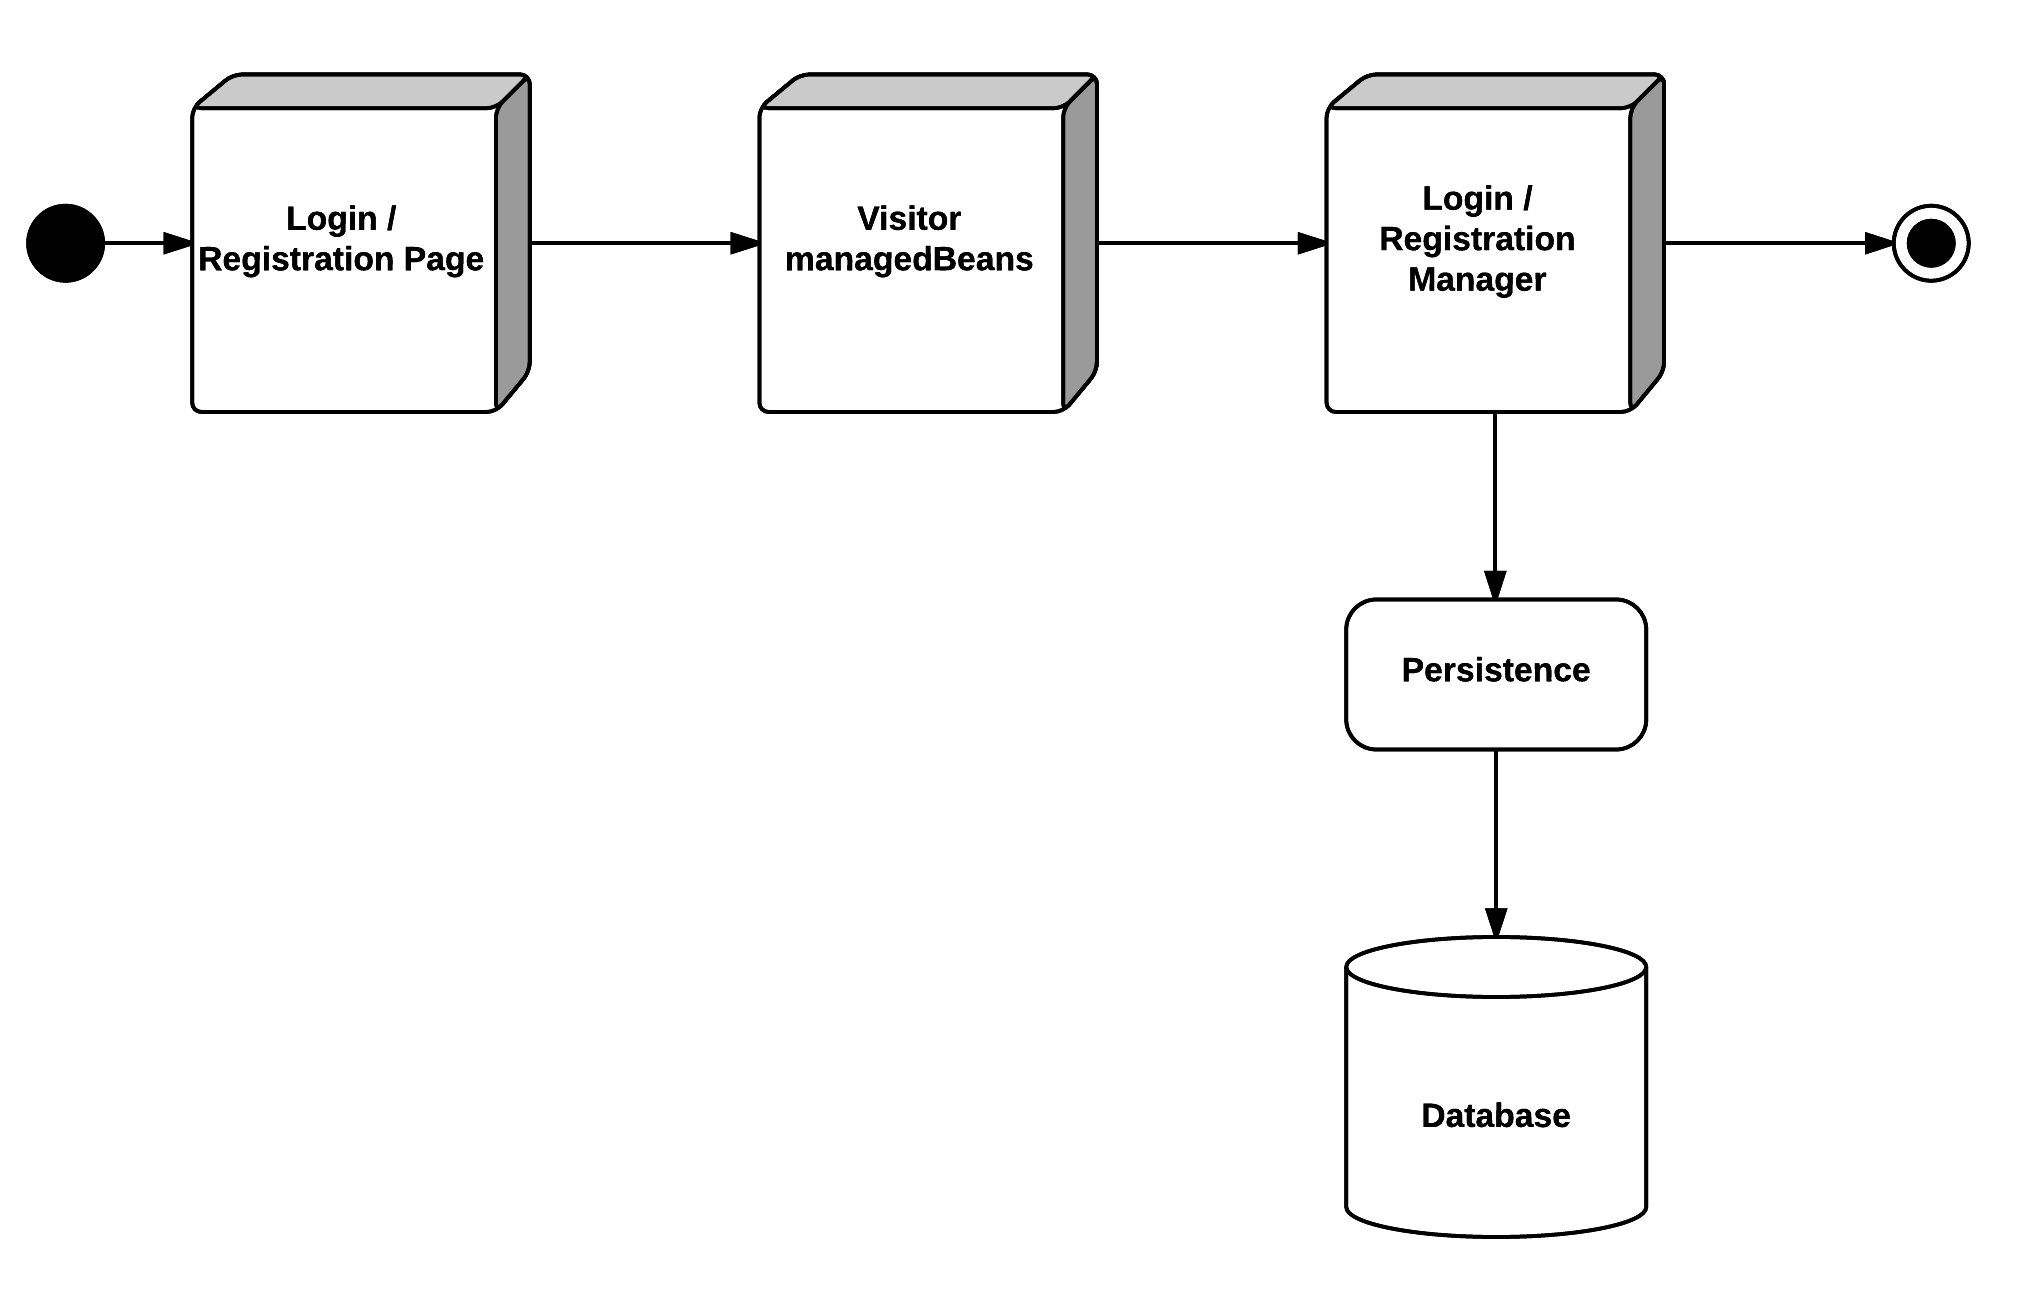
\includegraphics[width=\textwidth]{cpt/img/RuntimeLoginRegisterView}
	\caption{Runtime Login and Registration}
	\end{figure}
	\clearpage
	
	\item This diagram represent the components that are interested in the start taxi ride activity, and their interaction.
	\begin{figure}[htbp]
	\centering
	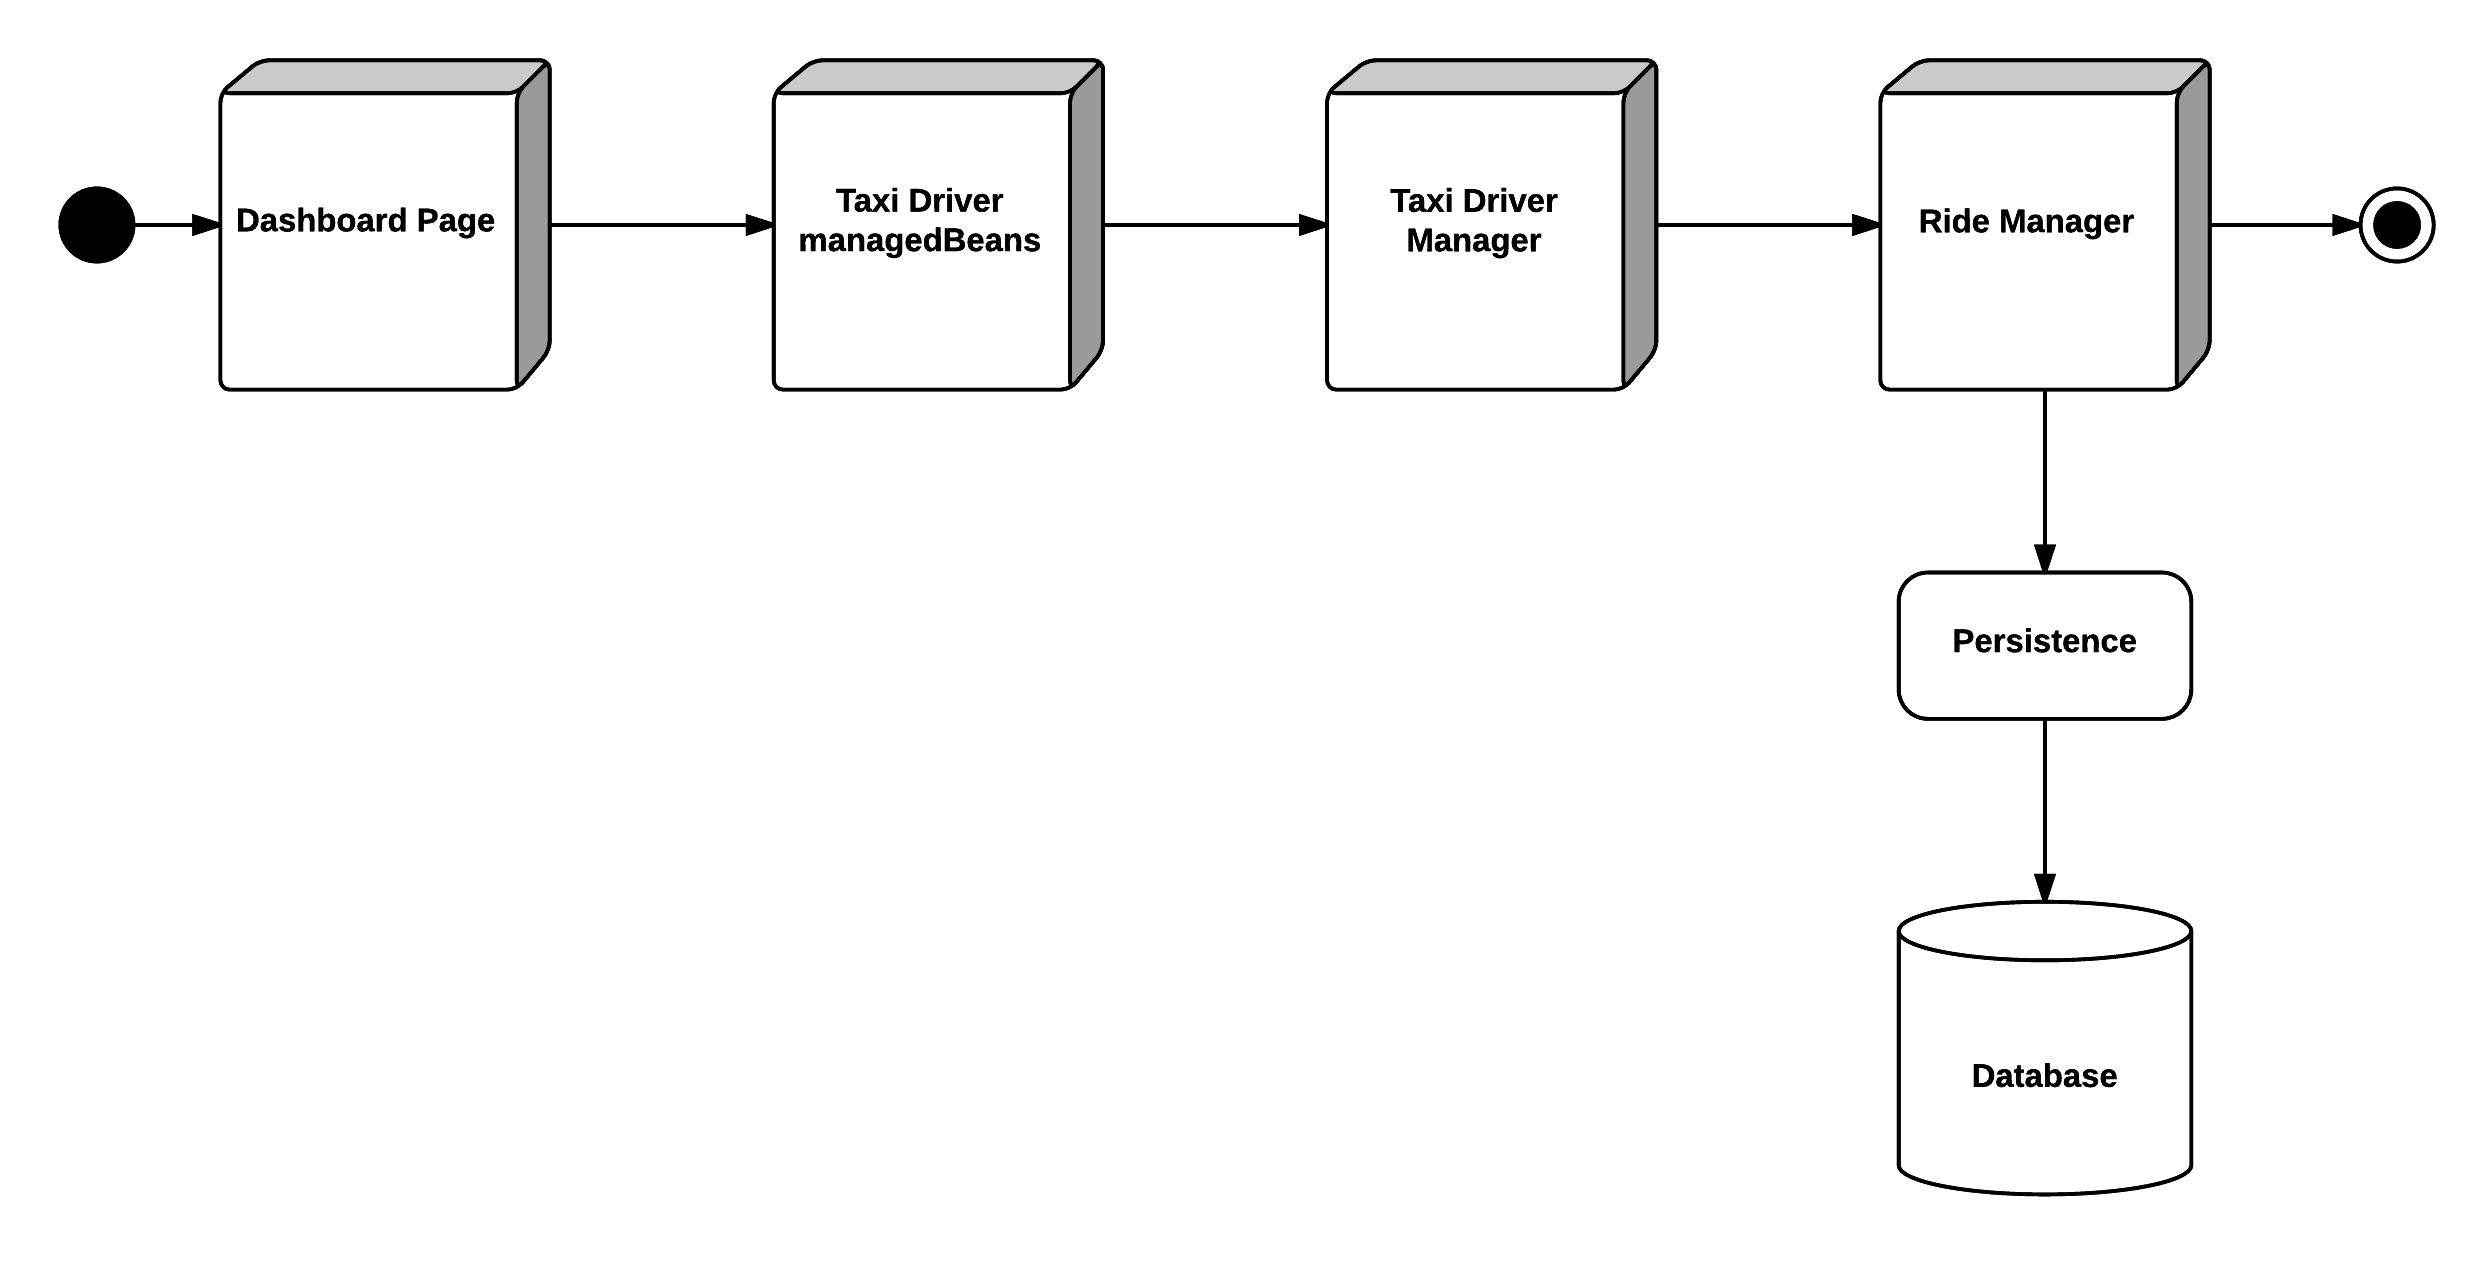
\includegraphics[width=\textwidth]{cpt/img/RuntimeStartTaxiRideView}
	\caption{Runtime start Taxi Ride}
	\end{figure}
	\clearpage
	
	\item This diagram represent the components that are interested in the summary activity, and their interaction.
	\begin{figure}[htbp]
	\centering
	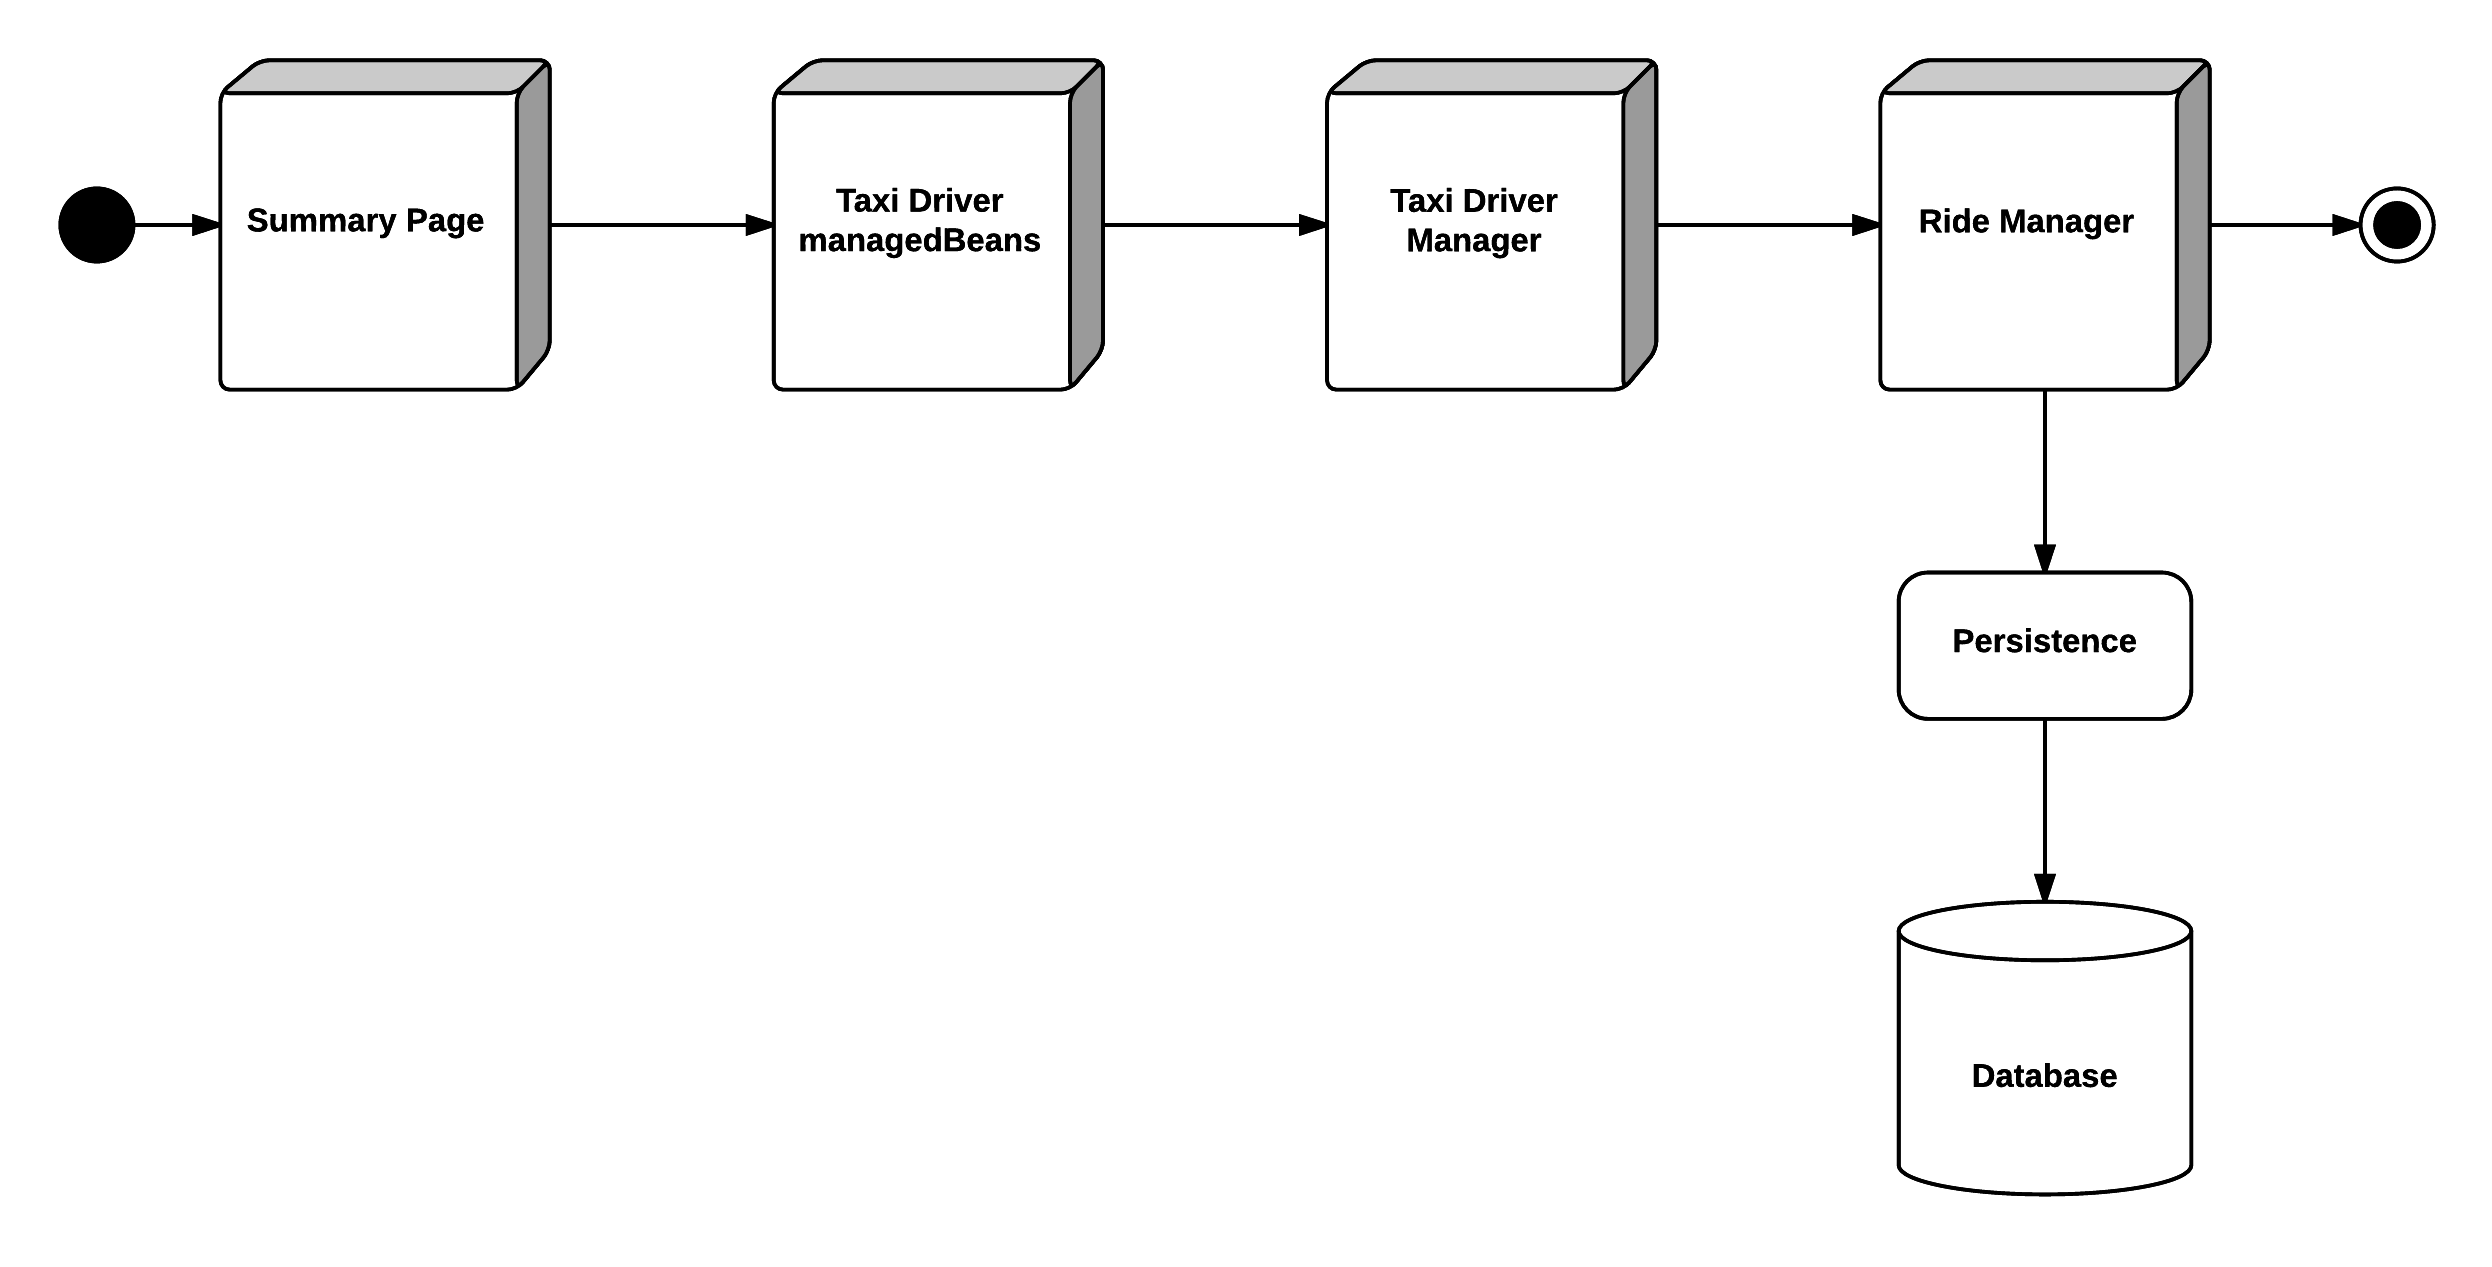
\includegraphics[width=\textwidth]{cpt/img/RuntimeSummaryView}
	\caption{Runtime Summary}
	\end{figure}
	\clearpage

\end{itemize}

\section{Component Interfaces}

\section{Selected Architectural Styles and Patterns}

\section{Other Design Decisions}